\documentclass[12pt,oneside]{article}

%%%%%%%%%%%%%%%%%%%%%%%%%%%%
%%   Zusaetzliche Pakete  %%
%%%%%%%%%%%%%%%%%%%%%%%%%%%%
\usepackage{enumerate}  
\usepackage{fancyhdr}
\usepackage{a4wide}
\usepackage{graphicx}
\usepackage{palatino}
\usepackage{multirow}
\usepackage{booktabs}
\usepackage{titlesec}
\usepackage{listings}
\usepackage{acronym}% http://ctan.org/pkg/acronym
\usepackage{enumitem}% http://ctan.org/pkg/enumitem
\usepackage{xcolor}
\usepackage[normalem]{ulem}
\usepackage{amsmath}
\usepackage{tikz}
\usetikzlibrary{positioning}
\usepackage{multirow}

%folgende Zeile auskommentieren für englische Arbeiten
\usepackage[ngerman]{babel}
%folgende Zeile auskommentieren für deutsche Arbeiten
%\usepackage[ngerman, english]{babel}

\usepackage[T1]{fontenc}
\usepackage[utf8]{inputenc}
\usepackage[bookmarks]{hyperref}
\usepackage[justification=centering]{caption}
\usepackage[style=trad-abbrv,backend=biber,natbib=true,maxbibnames=20]{biblatex}
\usepackage{csquotes}
\addbibresource{literatur.bib}

\setlength{\parindent}{0em} 
\setlist[itemize]{noitemsep, topsep=0pt}
\setlist[enumerate]{noitemsep, topsep=0pt}

\graphicspath{{./figs/}}

%%%%%%%%%%%%%%%%%%%%%%%%%%%%%%
%% Definition der Kopfzeile %%
%%%%%%%%%%%%%%%%%%%%%%%%%%%%%%

\pagestyle{fancy}
\fancyhf{}
\cfoot{\thepage}
\setlength{\headheight}{16pt}

%%%%%%%%%%%%%%%%%%%%%%%%%%%%%%%%%%%%%%%%%%%%%%%%%%%%%
%%  Definition des Deckblattes und der Titelseite  %%
%%%%%%%%%%%%%%%%%%%%%%%%%%%%%%%%%%%%%%%%%%%%%%%%%%%%%

\newcommand{\JMUTitle}[9]{

  \thispagestyle{empty}
  \vspace*{\stretch{1}}
  {\parindent0cm
  \rule{\linewidth}{.7ex}}
  \begin{flushright}
    \vspace*{\stretch{1}}
    \sffamily\bfseries\Huge
    #1\\
    \vspace*{\stretch{1}}
    \sffamily\bfseries\large
    #2\\
    \vspace*{\stretch{1}}
    \sffamily\bfseries\small
    #3
  \end{flushright}
  \rule{\linewidth}{.7ex}

  \vspace*{\stretch{1}}
  \begin{center}
    
\includegraphics[width=2in]{figs/2015_10_05_THB_FB-IM_Logo_RGB} \\
    \vspace*{\stretch{1}}
    \Large  Bachelorarbeit\\

    \vspace*{\stretch{2}}
   \large Fachbereich Informatik\\
    \large und Medien\\
    \large Technische Hochschule Brandenburg\\
    \vspace*{\stretch{1}}
    \large Betreuer:  #8 \\[1mm]
    \large 2. Betreuer:  #9 \\[1mm]
    
    \vspace*{\stretch{1}}
    \large Brandenburg, den #7 \\
        \vspace*{\stretch{0.25}}

    Bearbeitungszeit: 16.12.2021 - 16.02.2022 % Die Bearbeitungszeit der Seminar-/ Abschlussarbeit ist hier einzutragen.

  \end{center}
}

\titlespacing*{\section}
{0pt}{3.5ex plus 1ex minus .2ex}{.2ex plus .2ex}
\titlespacing*{\subsection}
{0pt}{1.5ex plus 1ex minus .2ex}{.2ex plus .2ex}
\titlespacing*{\subsubsection}
{0pt}{1.5ex plus 1ex minus .2ex}{.2ex plus .2ex}


\definecolor{mygreen}{rgb}{0,0.6,0}
\definecolor{mygray}{rgb}{0.5,0.5,0.5}
\definecolor{mymauve}{rgb}{0.58,0,0.82}

\lstset{ 
  backgroundcolor=\color{white},   % choose the background color; you must add \usepackage{color} or \usepackage{xcolor}; should come as last argument
  basicstyle=\footnotesize,        % the size of the fonts that are used for the code
  breakatwhitespace=false,         % sets if automatic breaks should only happen at whitespace
  breaklines=true,                 % sets automatic line breaking
  captionpos=b,                    % sets the caption-position to bottom
  commentstyle=\color{mygreen},    % comment style
  deletekeywords={...},            % if you want to delete keywords from the given language
  %escapeinside={\%*}{*)},          % if you want to add LaTeX within your code
  extendedchars=true,              % lets you use non-ASCII characters; for 8-bits encodings only, does not work with UTF-8
  %firstnumber=1000,                % start line enumeration with line 1000
  frame=single,	                   % adds a frame around the code
  keepspaces=true,                 % keeps spaces in text, useful for keeping indentation of code (possibly needs columns=flexible)
  keywordstyle=\color{blue},       % keyword style
  %language=Octave,                 % the language of the code
  morekeywords={*,...},            % if you want to add more keywords to the set
  numbers=left,                    % where to put the line-numbers; possible values are (none, left, right)
  numbersep=5pt,                   % how far the line-numbers are from the code
  numberstyle=\tiny\color{mygray}, % the style that is used for the line-numbers
  rulecolor=\color{black},         % if not set, the frame-color may be changed on line-breaks within not-black text (e.g. comments (green here))
  showspaces=false,                % show spaces everywhere adding particular underscores; it overrides 'showstringspaces'
  showstringspaces=false,          % underline spaces within strings only
  showtabs=false,                  % show tabs within strings adding particular underscores
  stepnumber=5,                    % the step between two line-numbers. If it's 1, each line will be numbered
  stringstyle=\color{mymauve},     % string literal style
  tabsize=2,	                   % sets default tabsize to 2 spaces
  %title=\lstname,                 %% show the filename of files included with \lstinputlisting; also try caption instead of title
  firstnumber=1,
}


\lstdefinelanguage{pddl}
{
    alsoletter=-,
    keywords={
        define,
    },
    morekeywords={[2]
        domain,
        problem,
        requirements,
        predicates,
        types,
        objects,
        action,
        durative-action,
        init,
        goal,
    },
    morekeywords={[3]
        parameters,
        vars,
        precondition,
        effect,
        condition,
        duration,
    },
    morekeywords={[4]
        forall,
        or,
        and,
        not,
        when,
        =,
        exists,
        imply,
        at,
        start,
        end,
        over,
        all,
    },
    comment=[l]{\;},
    sensitive=true
}[keywords, comments]


%%%%%%%%%%%%%%%%%%%%%%%%%%%%
%%  Beginn des Dokuments  %%
%%%%%%%%%%%%%%%%%%%%%%%%%%%%

\begin{document}

  \JMUTitle
      {Inbetriebnahme des OpenMANIPULATOR-X und Handlungsplanung mit\\ Partial Order Planning Forward}        % Titel der Arbeit
      {Fabian Claus}                        % Vor- und Nachname des Autors
      {20130004}
      
      {Technische Hochschule Brandenburg}  % Name der Fakultaet
      {Brandenburg 2021}                          % Ort und Jahr der Erstellung
      {13.01.2022}                              % Tag der Abgabe
      {Prof. Dr. Jochen Heinsohn}               % Name des Erstgutachters
      {Dipl. Inform. Ingo Boersch}                          % Name des Zweitgutachters

  \clearpage

  \thispagestyle{empty}

\large
\begin{flushright}
  Brandenburg, den 13.01.2022
\end{flushright}

\vspace*{50mm}
Ich, {\scshape Fabian Claus}, Student im Studiengang Informatik der
Technischen Hochschule Brandenburg, versichere an Eides statt, dass die vorliegende
Abschlussarbeit selbstständig verfasst und nicht mit anderen als den
angegebenen Hilfsmitteln erstellt wurde.

Sie wurde in dieser oder ähnlicher Form noch keiner Prüfungskommission
vorgelegt.\\

\vspace*{50mm}

\begin{flushright}
  {\scshape Fabian Claus}
\end{flushright}

\normalsize
  \thispagestyle{empty}

\begin{center}
    \Huge
    \textbf{Danksagung}
\end{center}

\vspace*{20mm}
\large
An dieser Stelle möchte ich mich bei all denjenigen bedanken, die mich während der Anfertigung dieser Bachelorarbeit unterstützt und motiviert haben.\\


Zuerst gebührt mein Dank Prof. Dr. Jochen Heinsohn und Dipl. Inform. Ingo Boersch, die meine Bachelorarbeit betreut und begutachtet haben.
Für die hilfreichen Anregungen und die konstruktive Kritik bei der Themenfindung und der Erstellung dieser Arbeit möchte ich mich herzlich bedanken.\\


Ich bedanke mich bei meiner Familie, die mich besonders bei den sprachlichen Aspekten dieser Arbeit unterstützt hat.
Ebenfalls möchte ich mich bei meinen Freunden bedanken, die mir bei der formalen und strukturellen Gestaltung zur Seite standen.\\


Vielen Dank!

\normalsize
  \lhead{}
  \pagenumbering{Roman}
  \setcounter{page}{1}

  \tableofcontents
  \clearpage
%%%%%%%%%%%%%%%%%%%%%%%%%%%%
%%  Kurzzusammenfassung   %%
%%%%%%%%%%%%%%%%%%%%%%%%%%%%
%\lhead{Zusammenfassung}
%\section*{Zusammenfassung}
%\addcontentsline{toc}{section}{Zusammenfassung}

%Eine Kurzzusammenfassung der Vorgehensweise und der wesentlichen Ergebnisse.

%Allgemeine Merkmale
%\begin{itemize}
%    \item Objektivität: Es soll sich jeder persönlichen Wertung enthalten.
%    \item Kürze: Es soll so kurz wie möglich sein.
%    \item Verständlichkeit: Es weist eine klare, nachvollziehbare Sprache und Struktur auf.
%    \item Vollständigkeit: Alle wesentlichen Sachverhalte sollen enthalten sein.
%    \item Genauigkeit: Es soll genau die Inhalte und die Meinung der Originalarbeit wiedergeben.
%\end{itemize}{}

%\newpage
\lhead{Abbildungsverzeichnis} % Bei englischsprachiger Arbeit anzupassen auf: List of Figures
\addcontentsline{toc}{section}{Abbildungsverzeichnis} % Bei englischsprachiger Arbeit anzupassen auf: List of Figures
\listoffigures

\newpage
\lhead{Tabellenverzeichnis} % Bei englischsprachiger Arbeit anzupassen auf: List of Tables
\addcontentsline{toc}{section}{Tabellenverzeichnis} % Bei englischsprachiger Arbeit anzupassen auf: List of Tables
\listoftables
\newpage

\setlength{\parskip}{0.5em} 


%%%%%%%%%%%%%%%%%%%%%%%%%%%%%%%%%%
%%  Definition der Abkürzungen  %%
%%%%%%%%%%%%%%%%%%%%%%%%%%%%%%%%%%
\lhead{Abkürzungsverzeichnis} % Bei englischsprachiger Arbeit anzupassen auf: List of Abbreviations
\section*{Abkürzungsverzeichnis} % Bei englischsprachiger Arbeit anzupassen auf: List of Abbreviations
\addcontentsline{toc}{section}{Abkürzungsverzeichnis} % Bei englischsprachiger Arbeit anzupassen auf: List of Abbreviations

\acrodefplural{RCL}{ROS Client Libraries}

\begin{acronym}
\acro{IDL}{Interface Definition Language}
\acro {PDDL}{Planning Domain Definition Language}
\acro{RCL}{ROS Client Library}
\acro{ROS2}{Robot Operating System 2}
 \acro{VM}{Virtuelle Maschine}

\acro{ML}{Machine Learning}
\end{acronym}


%%%%%%%%%%%%%%%%%%%%%%%%%%%%
%%  Einstellungen  %%
%%%%%%%%%%%%%%%%%%%%%%%%%%%%
\clearpage
\pagenumbering{arabic}  
    \setcounter{page}{1}
\lhead{\nouppercase{\leftmark}}

%%%%%%%%%%%%%%%%%%%%%%%%%%%%
%%  Hauptteil  %%
%%%%%%%%%%%%%%%%%%%%%%%%%%%%
%\section{TODOS}
\begin{itemize}
    \item Neues Bild für Keyboard Teleop \ref{teleop}
    \item \sout{Bilder für Teleop Posen}
    \item Bild für Servo Abdeckung vorgestanzt
    \item Überprüfen ob all Anhänge aktuell sind
    \item Entscheidung Bezeichnung für OMX, Abk., Greifarm, OpenManipulator-X, OpenMANIPULATOR-X
    \item \sout{Fehlersuche Abstürze PlanSys2}
    \item \sout{Zusammenfassen der Gripper Nodes zu einer parametrisierten Node}
    \item baudrate änderungen für omx controller dokumentieren
    \item code kommentieren
    \item launch file für eigenes package beschreiben
    \item \sout{Move node umschreiben um pair anstelle mehrer maps zu nutzen}
    \item PKG readme anpassen: start befehle sowie problem
    \item \sout{domänen dateien aufräumen, umbenennen}
    \item Bilder für PlanSys2 Terminal
    \item section struktur für ROS2 überdenken
    \item aspect ratio für Bilder fixen
    \item Erklärung von durative actions von Implementierung zu Grundlagen verschieben
    \item Angabe Author für simmons\_2001
    \item einheitlich Knoten oder Nodes, Leaf/ Blatt
    \item Eltern /Kind Knoten oder Vorgänger Nachfolger
    \item Quellenplatzierung (bei Aufzählungen)
    \item quellenangabe tabellen
    \item grafiken für bt
    \item tabelle mit bt symbolen
\end{itemize}
\section{Einleitung} \label{einleitung}
Dieser Teil der Arbeit sollte folgende Inhalte haben:

\begin{itemize}
\item Einführung in die Problemstellung
\item Motivation und Herleitung des Themas
\item Aufbau der Arbeit
\end{itemize}

Hinweis:
Es hat sich als hilfreich erwiesen, die Einleitung mit der Zusammenfassung bzw.\ dem Abstract und der Schlussfolgerung zu vergleichen.
Damit stellt man sicher, dass diese inhaltlich im Bezug auf Zielsetzung und Motivation übereinstimmen.
Der Umfang sollte ca.\ 5 \% der gesamten Arbeit betragen.
\\
\\
Roboter sind ein wichtiger Bestandteil der Forschung und der Lehre.
Auch im Fachbereich Informatik und Medien der \ac{THB} sind Roboter Teil und Kern mehrerer Module.
Aktuell werden hier das an der \ac{THB} entwickelte AKSEN-Board~\footnote{http://ots.th-brandenburg.de/aksen-controller-fur-reaktive-roboter.html} in Kombination mit LEGO sowie Pioneer 2/3 Roboter~\footnote{http://ots.th-brandenburg.de/pioneer2-und-pioneer3roboter.html} genutzt.
Zukünftig sollen auch der \ac{ROS2} basierte Roboter TurtleBot3 Waffle Pi~\footnote{https://emanual.robotis.com/docs/en/platform/turtlebot3/overview/} mit dem Greifarm OMX genutzt werden.\\
In dieser Arbeit soll, speziell für den OMX, ein erster Überblick über die grundsätzlichen Vorgänge und Prozesse bei dessen Nutzung gegeben werden.

\subsection{Aufgabe}
Im Rahmen der Bachelorarbeit soll der Greifarm OpenMANIPULATOR-X der Firma Robotis in Betrieb genommen sowie die Möglichkeiten der Steuerung erprobt werden.
Weiterhin soll die Steuerung Mittels Handlungsplanung ermöglicht werden.
Hierfür sind bestehende Bibliotheken und Frameworks zu evaluieren und ein ausgewähltes zu implementieren und an einem praktischen Beispiel zu demonstrieren.
Für das gewählte Framework oder den gewählten Planer sollen verschiedene Szenarien getestet werden, die die Möglichkeiten und Grenzen zeigen.
Es soll ein ROS2 Package erstellt werden, mithilfe dessen der Einstieg in die Nutzung des OMX vereinfacht werden soll.
Abschließend sollen Möglichkeiten der Einbindung in den Lehrbetrieb gezeigt werden.
\subsection{Abgrenzung/Motivation}


\section {Grundlagen}
In diesem Abschnitt wird zunächst der Greifarm OpenMANIPULATOR-X vorgestellt.
Anschließend wird eine Übersicht über die wichtigsten Komponenten des Betriebssystems gegeben, mit dem dieser Greifarm läuft.
Weiterhin werden die theoretischen Grundlagen der Planung dargestellt, die zur Steuerung des Greifarms genutzt werden sollen.
Abschließend wird das System erklärt, das Planung und Roboter kombiniert.
\subsection{OpenMANIPULATOR-X}
Der OpenMANIPULATOR-X ist ein von der Firma ROBOTIS{\footnote{http://en.robotis.com}} nach den Prinzipien ``OpenSoftware`` und ``OpenHardware`` hergestellter Greifarm.
OpenSoftware steht hierbei dafür, dass es ein OpenSource Projekt ist und auf dem OpenSource Projekt \ac{ROS2} basiert.
OpenHardware steht dafür, dass die meisten Komponenten als STL-Dateien zur Verfügung stehen und als Ersatzteile oder zum Anpassen des Greifarms mittels eines 3D-Druckers selbst hergestellt werden können.\\
Der OpenMANIPULATOR-X ist eine 5DOF (5 Degrees of Freedom) Plattform, welche mittels 5 Servomotoren{\footnote{Modelbezeichnung: DYNAMIXEL XM430-W350-T}} gesteuert wird.
Dies ist aufgeteilt in 4DOF für den Arm sowie 1DOF für den Greifer.
Es kann eine Last bis 500g getragen werden.
\subsection{ROS2}
\ac{ROS2} ist eine Sammlung von Bibliotheken und Werkzeugen für Robotik-Applikationen welche alle OpenSource sind.
Die erste \ac{ROS2} Release-Version erschien im Dezember 2017 unter dem Namen ''Ardent Apalon''.\\
Es werden  mehrere \acp{RCL}  zur Verfügung gestellt, welche den Zugriff auf die \ac{ROS2}-API ermöglichen.
Die \acp{RCL} für die Sprachen C++ und Python (rclcpp und rclpy) werden dabei direkt vom \ac{ROS2}-Team verwaltet.
Von der Community wurden weitere \acp{RCL}, unter anderem für die Sprachen C\#, Swift und Rust, entwickelt.\\
Um die Entwicklung der \acp{RCL} zu vereinfachen und die Logik sprachunabhängig zu machen werden Funktionalitäten als C Interfaces zugänglich gemacht, für welche in den \acp{RCL} Wrapper geschrieben werden.\\
Die grundlegende Komponente einer \ac{ROS2} Anwendung ist die Node.
Typischerweise besteht eine Anwendung aus mehreren Nodes.
Entsprechend dem Prinzip \emph{Separation of Concerns} (Trennung der Zuständigkeiten) sollen Nodes so implementiert werden, dass sie jeweils nur eine spezifische Aufgabe haben.
\subsubsection{Interfaces}
In diesem Abschnitt werden die verschiedenen Arten von Interfaces beschrieben, die für die im folgenden Abschnitt~\ref{rosnodecomm} erklärten Methoden zur Kommunikation zwischen mehreren Nodes genutzt werden.\\
\ac{ROS2}-Interfaces definieren, welche Daten gesendet werden und welchen Datentyp diese haben.
Sie werden in der \ac{IDL} geschrieben, die es ermöglicht automatisch Source Code in verschiedenen Sprachen für diese zu generieren.\\

\textbf{Message} Eine Message ist die einfachste Art der \ac{ROS2}-Interfaces, die gleichzeitig auch ein Baustein für die anderen Interfaces sein wird.\\
Message-Definitionen haben die Dateiendung \verb|.msg| und werden per Konvention in einem Ordner \verb|msg/| gespeichert.
Jede \verb|.msg| Datei besteht aus den folgenden Teilen:
\begin{itemize}
\item Felder
\item Konstanten
\end{itemize}
Konstanten sind optional und es gibt mindestens ein Feld.
Jedes Feld besteht aus einem Datentyp und einem durch ein Leerzeichen getrennten Namen: \verb|typ name|, z.B. \verb|bool isDone|.
Als Datentyp können dabei die integrierten Datentypen (s. Tabelle~\ref{tab:builtintypes}) oder der Name anderer Messages genutzt werden.
Zusätzlich kann jeder integrierte Datentyp als Array definiert werden (s. Tabelle~\ref{tab:arraytypes}).\\
Feldnamen müssen kleingeschrieben sein.
Es können alphanumerische Zeichen sowie der Unterstrich zur Trennung von Wörtern genutzt werden.
Das erste Zeichen muss ein Buchstabe sein und der Name darf nicht mit einem Unterstrich enden.
Zusätzlich darf es keine aufeinander folgende Unterstriche geben.\\
Konstanten behalten das Format der Felder bei.
Der Name der Konstante wird komplett in Großbuchstaben geschrieben.
Zusätzlich bekommen Konstanten einen Wert zugewiesen, welcher nicht innerhalb des Programms geändert werden kann.
Die Zuweisung des Wertes erfolgt mit dem ''\verb|=|'' Zeichen: \verb|string EXAMPLE="test"|.
\begin{table}[ht]
    \centering
    \caption{Integrierte Datentypen für Interfaces und deren C++ Equivalent}
\begin{tabular}{|l|l|}
\hline
\textbf{Typ} & \textbf{C++}   \\ \hline
bool         & bool           \\ \hline
byte         & uint8\_t       \\ \hline
char         & char           \\ \hline
float32      & float          \\ \hline
float64      & double         \\ \hline
int8         & int8\_t        \\ \hline
uint8        & uint8\_t       \\ \hline
int16        & int16\_t       \\ \hline
uint16       & uint16\_t      \\ \hline
int32        & int32\_t       \\ \hline
uint32       & uint32\_t      \\ \hline
int64        & int64\_t       \\ \hline
uint64       & uint64\_t      \\ \hline
string       & std::string    \\ \hline
wstring      & std::u16string \\ \hline
\end{tabular}
    \label{tab:builtintypes}
\end{table}
\begin{table}[ht]
    \centering
    \caption{Array Typen und deren C++ Equivalent}
\begin{tabular}{|l|l|}
\hline
\textbf{Typ} & \textbf{C++}   \\ \hline
static array               & std::array<T, N>   \\ \hline
unbounded dynamic array    & std::vector        \\ \hline
bounded dynamic array      & custom\_class<T, N> \\ \hline
bounded string             & std::string        \\ \hline
\end{tabular}
    \label{tab:arraytypes}
\end{table}

\textbf{Service} Service-Definitionen beschreiben eine Anfrage und eine Antwort.
Die Definition hat die Dateiendung \verb|.srv| und wird im Ordner \verb|srv/| gespeichert.
Anfrage und Antwort werden innerhalb der Datei durch ''\verb|---|'' getrennt.
Für beide Teile gilt, dass sie gültig sind, wenn sie einer gültigen Message-Definition entsprechen.
Ein Beispiel einer einfachen Service-Definition ist in Listing~\ref{lst:serviceexample} gegeben.\\
\begin{minipage}{\linewidth}%minipage to prevent page break
\begin{lstlisting}[caption={Beispiel einer Service-Definition}, label={lst:serviceexample}]
int32 request_int
string request_string
---
float32 response_float
\end{lstlisting}
\end{minipage}

\textbf{Action} Action-Definitionen bestehen aus den 3 Teilen Anfrage, Antwort und Feedback, in dieser Reihenfolge.
Wie auch für Service-Definitionen gilt, dass die Teile durch ''\verb|---|'' getrennt sind und jeder einzelne Teil gültig ist, wenn er einer gültigen Message-Definition entspricht.

\subsubsection{Node-Kommunikation}{\label{rosnodecomm}}
Damit verschiedene Nodes untereinander kommunizieren können, gibt es verschiedene Methoden, die sich darin unterscheiden, in welche Richtungen Nachrichten gesendet werden und ob es eine direkte Reaktion gibt.
Für alle Methoden gilt, dass sie von einer Node unter einem bestimmten Namen sowie einem Typ zur Verfügung gestellt werden und von anderen Nodes durch eben diese genutzt werden können.\\

\textbf{Topic} Topics entsprechen in etwa einem Newsletter System: eine Node veröffentlicht Daten (Publisher), welche von allen anderen Nodes (Subscriber) empfangen werden, die sich für diese registriert haben (s. Abbildung~\ref{fig:topic}).
Das Format der Daten entspricht einer gewählten Message-Definition.\\

\begin{figure}[ht!]
    \centering
    \begin{tikzpicture}[node distance=5cm,every node/.style={circle, draw, minimum size=1.5cm}]

    \node (1) at (0,0) [text width=2cm,align=center,circle,draw] {Publisher};
    \node (2) at (10,0) [text width=2cm,align=center,circle,draw,right of=1] {Subscriber};

    \path[-{latex},every node/.style={font=\sffamily\small}]
    (1) edge[bend left] node [midway,above] {Nachricht (Message)} (2)
    \end{tikzpicture}
    \caption{Nachrichtenfluss eines Topic}
    \label{fig:topic}
\end{figure}
\textbf{Service und Client} Services werden für Prozesse genutzt, in denen eine Anfrage gesendet und eine Antwort erwartet wird.
Ein Client sendet die Anfrage an den Service, der eine Antwort zurückgibt (s. Abbildung~\ref{fig:service}).
Als Typ wird eine Servicedefinition genutzt.\\

\begin{figure}[ht!]
    \centering
    \begin{tikzpicture}[node distance=5cm,every node/.style={circle, draw, minimum size=2cm}]

        \node (1) at (0,0) [text width=2cm,align=center,circle,draw] {Client};
        \node (2) at (10,0) [text width=2cm,align=center,circle,draw,right of=1] {Service};

        \path[-{latex},every node/.style={font=\sffamily\small}]
        (1) edge[bend left] node [midway,above] {Anfrage (Request)} (2)
        (2) edge[bend left] node [midway,below] {Antwort (Response)} (1)
    \end{tikzpicture}
    \caption{Nachrichtenfluss eines Service}
    \label{fig:service}
\end{figure}
\textbf{Action Server und Client} Actions sind für länger andauernde Prozesse gedacht.
Eine Node erstellt einen Action Server über welchen eine Action zur Verfügung gestellt wird.
Andere Nodes können über einen Action Client eine Anfrage senden.
Der Server bearbeitet die Anfrage und sendet bei Beendigung eine Antwort mit einem Ergebnis an den Client.
Während der Dauer der Action kann der Server den Client optional mit Feedback-Nachrichten über den aktuellen Status informieren.
Dieser Nachrichtenfluss wird in Abbildung~\ref{fig:action} gezeigt.\\
Als Typ wird eine Action Definition genutzt.\\
\begin{figure}[ht!]
    \centering
    \begin{tikzpicture}[node distance=5cm,every node/.style={circle, draw, minimum size=2cm}]

        \node (1) at (0,0) [text width=2cm,align=center,circle,draw] {Action Client};
        \node (2) at (10,0) [text width=2cm,align=center,circle,draw,right of=1] {Action Server};

        \path[-{latex},every node/.style={font=\sffamily\small}]
        (1) edge[bend left] node [midway,above] {Anfrage (Request)} (2)
        (2) edge[bend left] node [midway,below] {Antwort (Response)} (1)
        (2) edge[bend left=10] node [midway,below] {Feedback} (1)
    \end{tikzpicture}
    \caption{Nachrichtenfluss einer Action}
    \label{fig:action}
\end{figure}
\subsection {Planung}
Planung (auch Handlungsplanung) ist ein Bereich der Künstlichen Intelligenz, welcher sich mit der Lösung von Planungs- und Schedulingproblemen befasst~\cite{aiplanning}.
\subsubsection{Stanford Research Institute Problem Solver}{\label{chap:strips}}
Der \emph{\ac{STRIPS}} ist ein automatischer Planer, welcher von Richard Fikes und Nils Nilsson 1971 entwickelt wurde~\cite{FIKES1971189}.
Mit dem gleichen Namen wird auch die Sprache bezeichnet, welche als Eingabe für diesen Planer genutzt wird.
In diesem Abschnitt wird zunächst auf die Sprache eingegangen, welche die Grundlage vieler weiterer Sprachen zur Darstellung von Planungsdomänen und -problemen ist.
Anschließend wird der von \ac{STRIPS} genutzte Algorithmus beschrieben.\\
Ein \ac{STRIPS}-Modell besteht aus 3 Teilen:
\begin{itemize}
    \item Startzustand
    \item Ziele
    \item Aktionen
\end{itemize}
Aktionen bestehen wiederum aus:
\begin{itemize}
    \item Vorbedingungen
    \item Effekten
\end{itemize}
Ein \ac{STRIPS}-Modell kann mathematisch als 4-Tupel \((P,O,I,G)\) beschrieben werden \cite{stripsdef}:
\begin{enumerate}
    \item \(P\): eine endliche Menge von Bedingungen
    \item \(O\): eine endliche Menge von Aktionen (auch Operatoren) mit der Form $Pre \Rightarrow Post$:
    \item \(I\): der Startzustand, $I\subseteq P$
    \item \(G\): eine endliche Menge von Zielen
\end{enumerate}
Es gilt die \emph{Closed World Assumption (CWA)}: alles was nicht explizit als wahr beschrieben ist, gilt als falsch.\\
$P$ ist die Menge aller Bedingungen, die relevant sind.
Jeder Zustand ist eine Teilmenge $S\subseteq P$.\\
$O$ ist die Menge der Aktionen die einen Zustand in einen anderen ändern können.
Aktionen sind 4-Tupel \((o^+,o^-,o_+,o_-)\), bei dem jedes Element eine Menge von Bedingungen sind.
Die ersten zwei Mengen beschreiben die Vorbedingungen ($Pre$): Bedingungen, die wahr sein müssen ($o^+$) sowie Bedingungen, die falsch sein müssen ($o^-$).
Die letzten beiden Mengen beschreiben den Effekt, den die Aktion nach ihrer Ausführung auf einen Zustand hat ($Post$): Bedingungen, die wahr werden ($o_+$) und Bedingungen, die falsch werden ($o_-$).\\
$I$ beschreibt, welche Bedingungen anfangs wahr oder falsch sind.
Eine Bedingung $p\in P$ ist anfangs wahr, wenn $p\in I$ und sonst falsch.\\
$G$ ist die Menge der Bedingungen, die erreicht werden soll, bestehend aus den Zielen, die wahr sein sollen ($G_+$) und denen, die falsch sein sollen ($G_-$).
Ein Zustand $S\subseteq P$  ist ein Zielzustand, wenn $G_+\subseteq S$ und $G_-\cap S =\emptyset$.\\
Ein Plan besteht aus einer Menge von Aktionen, die vom Startzustand zu einem Zielzustand führen.
Dieser Plan ist ein \emph{Total-Order} Plan: alle Aktionen haben eine feste Reihenfolge innerhalb des Plans.
Um einen Plan zu finden, wird ein Suchbaum erstellt.
Die Suche findet im Zustandsraum statt.
Jeder Knoten ist ein Zustand.
Jede Kante ist die Aktion, um den Zustand bzw. Knoten, von der die Kante ausgeht, zu dem Zustand zu überführen, zu dem die Kante geht.
Es wird die GPS Strategie angewandt, um Unterschiede zwischen dem aktuellen Zustand und dem Ziel zu extrahieren und relevante Aktionen für diese Unterschiede zu finden~\cite{FIKES1971189}.\\
\ac{STRIPS} beginnt damit, das Ziel $G_0$ für den Startzustand $M_0$ zu beweisen.
Gelingt dies, ist das Ziel bereits erreicht und kein Plan notwendig.
Ist das Ziel nicht beweisbar, wird der Unterschied zwischen $M_0$ und $G_0$ ermittelt und von diesem aus weiter gesucht.
Es wird eine Aktion gesucht, die diesen Unterschied weiter verringern kann.
Vorbedingungen dieser Aktion werden als Unterziel genutzt.
Kann ein (Unter)Ziel für den Zustand $M_0$ bewiesen werden, werden die Effekte der Aktion auf $M_0$ angewandt und es entsteht ein Zustand $M_1$.
Dieses Verfahren wiederholt sich bis ein Zustand entsteht, in dem das Ziel $G_0$ bewiesen werden kann.
\subsubsection{Planning Domain Definition Language}
Die \emph{\ac{PDDL}} ist eine Sprache zur Modellierung von Planungsaufgaben.
Im Rahmen dieser Arbeit wird nicht auf alle Aspekte von \ac{PDDL} eingegangen.
Der Fokus liegt auf einigen grundlegenden Teilen sowie auf den genutzten Erweiterungen.\\
Die Beschreibung des Problems setzt sich aus folgenden grundlegenden Komponenten zusammen:
\begin{itemize}
    \item Objekt
    \item Prädikat
    \item Startzustand
    \item Aktion
    \item Ziel
\end{itemize}
Objekte sind Dinge in der Welt, die für die Planung relevant sind.
Dies können bspw.\ Orte oder Personen sein und werden in \ac{PDDL} entsprechend Listing~\ref{lst:pddlobjects} beschrieben.
\begin{lstlisting}[caption={Objektbeschreibung in PDDL},language=pddl,label={lst:pddlobjects}]
(:objects kitchen supermarket
          fabian)
\end{lstlisting}
Prädikate sind Eigenschaften, die Objekte haben können.
Eine Person kann sich an einem Ort befinden oder eine bestimmte Größe haben (s. Listing~\ref{lst:pddlpredicates}).
\begin{lstlisting}[caption={Prädikatbeschreibung in PDDL},language=pddl,label={lst:pddlpredicates}]
(:predicates (person_at ?person ?location)
            (tall ?person))
\end{lstlisting}
Der Startzustand ist die Beschreibung der Welt zu Beginn der Planungsaufgabe.
Er besteht aus einer Menge von Instanzen von Prädikaten, also Prädikate, die an Objekte gebunden sind (s. Listing~\ref{lst:pddlinit}).
\begin{lstlisting}[caption={Startzustand in PDDL},language=pddl,label={lst:pddlinit}]
(:init (person_at fabian kitchen))
\end{lstlisting}
Aktionen sind die vorhandenen Möglichkeiten, den Zustand der Welt zu verändern.
Diese entsprechen den in Abschnitt~\ref{chap:strips} beschriebenen Aktionen mit einer Menge von Vorbedingungen und einer Menge von Effekten (s. Listing \ref{lst:pddlaction}).
\begin{lstlisting}[caption={Aktion, um eine Person von einem Ort zum anderen zu bewegen in PDDL},language=pddl,label={lst:pddlaction}]
(:action move
    :parameters (?p ?loc_from ?loc_to)
    :precondition (and (person_at ?p ?loc_from))
    :effect (and (person_at ?p ?loc_to)
                (not (person_at ?p ?loc_from))))
\end{lstlisting}
Ein Ziel ist eine Menge von Instanzen, die am Ende der Planung Teil des Zustands der Welt sein soll (s. Listing~\ref{code:pddlgoal}).
\begin{lstlisting}[caption={Ziel in PDDL},language=pddl,label=code:pddlgoal]
(:goal (and (person_at fabian supermarket))
\end{lstlisting}
Diese Komponenten werden aufgeteilt:
\begin{itemize}
    \item Domäne
    \item Problem
\end{itemize}
Die Domäne enthält die allgemeinen Rahmenbedingungen für das Problem: Prädikate und Aktionen.
Die Datei beginnt mit \verb|(define (domain name_der_domäne)|.\\
Das Problem enthält die Informationen zu einem spezifischen Problem: Objekte, den Startzustand und das Ziel.
Die Datei beginnt mit\\\verb|(define (problem name_des_problems) (:domain name_der_domäne)|.\\
Um sicherzustellen, dass nur bestimmte Objekte für bestimmte Parameter in Frage kommen (es kann mit der \emph{move} Aktion nur eine Person bewegt werden und der Start und das Ziel sind Orte) wurden ursprünglich weitere Prädikate genutzt, um Objekte zu typisieren.
Für das aktuelle Beispiel wären das die Prädikate \emph{location(x)} und \emph{person(x)}.
Die Aktion \emph{move} wird dann um entsprechende Vorbedingungen erweitert (s. Listing~\ref{lst:pddlactiontypepredicates}).
\begin{lstlisting}[caption={Move Aktion mit Prädikaten zur Typisierung},language=pddl,label={lst:pddlactiontypepredicates}]
(:action move
    :parameters (?p ?loc_from ?loc_to)
    :precondition (and (person ?p)
                        (location ?loc_from)
                        (location ?loc_to)
                        (person_at ?p ?loc_from))
    :effect (and (person_at ?p ?loc_to)
                (not (person_at ?p ?loc_from))))
\end{lstlisting}
Um dies zu vereinfachen, wurde mit \ac{PDDL} 2.1 unter anderem direkte Typisierung eingeführt.
In der Domäne werden die möglichen Typen deklariert, Objekte werden mit einem Typ initialisert und Aktionen können Parameter auf einen Typ beschränken (s. Listing~\ref{lst:pddltypes})
\begin{lstlisting}[caption={Typ Unterstützung in \ac{PDDL} 2.1},language=pddl,label={lst:pddltypes}]
(:types person
        location)
(:objects kitchen supermarket - location
          fabian - person)
(:action move
    :parameters (?p - person ?loc_from - location ?loc_to - location)
    :precondition (and (person_at ?p ?loc_from))
    :effect (and (person_at ?p ?loc_to)
                (not (person_at ?p ?loc_from))))
\end{lstlisting}
Eine weitere Neuerung in \ac{PDDL} ist die \emph{durative action} zur Modellierung von Aktionen mit einer Dauer für das temporale Planen.\\

\subsubsection{PDDL-Plugin für VS Code}
- nach Implementierung verschieben?\\
Im Marketplace von Visual Studio Code ist ein PDDL-Plugin von Jan Dolejsi verfügbar.
Dieses vereinfacht die Entwicklung und das Testen von Domänen und Problemen im PDDL Format.
Es beinhaltet Syntax-Highlighting und Snippets, sowie die Möglichkeit direkt Pläne zu suchen und zu visualisieren.
Um Pläne mit \ac{POPF} zu suchen, muss der Planer in der Overview-Page des Plugins hinzugefügt werden.
Der Pfad zum \ac{POPF}-Planer ist: \emph{/opt/ros/foxy/lib/popf/popf}.\\
Über das Kontext-Menü einer Domänen- oder Problemdatei lässt sich der Planer starten und es erfolgt eine Ausgabe in der Konsole (s. Abbildung~\ref{fig:pluginplan}) sowie eine Visualisierung wenn ein Plan gefunden wurde (s. Abbildung~\ref{fig:pluginvis}).
Der zeitliche Ablauf wird in der Abbildung von links nach rechts dargestellt.
Alle Aktionen werden farblich markiert, wobei eine Aktion auch bei mehrfacher Ausführung die gleiche Farbe erhält.
Im oberen Abschnitt gibt es eine einfache Übersicht des Plans: welche Aktionen wurden wann ausgeführt und mit welchen Parametern.
Im unteren Abschnitt wird dargestellt, welche Instanzen zu welchem Zeitpunkt als Teil welcher Aktion genutzt wurden.
\begin{figure}[ht!]
    \centering
    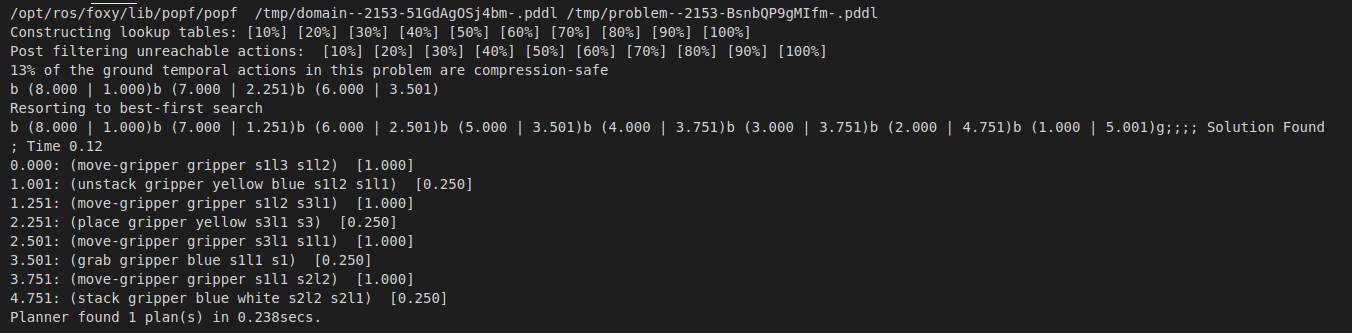
\includegraphics[width=\textwidth]{plugin_plan}
    \caption{Konsolenausgabe nach Ausführung des Planers über das PDDL-Plugin}
    \label{fig:pluginplan}
\end{figure}

\begin{figure}[ht!]
    \centering
    \begin{minipage}[t]{0.45\linewidth}
        \centering
        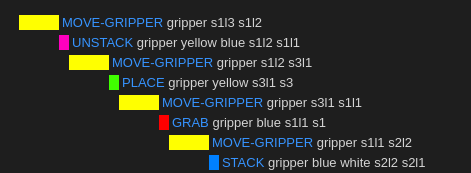
\includegraphics[width=\linewidth,keepaspectratio]{plugin_vis1}
    \end{minipage}% <- sonst wird hier ein Leerzeichen eingefügt
    \hfill
    \begin{minipage}[t]{0.45\linewidth}
        \centering
        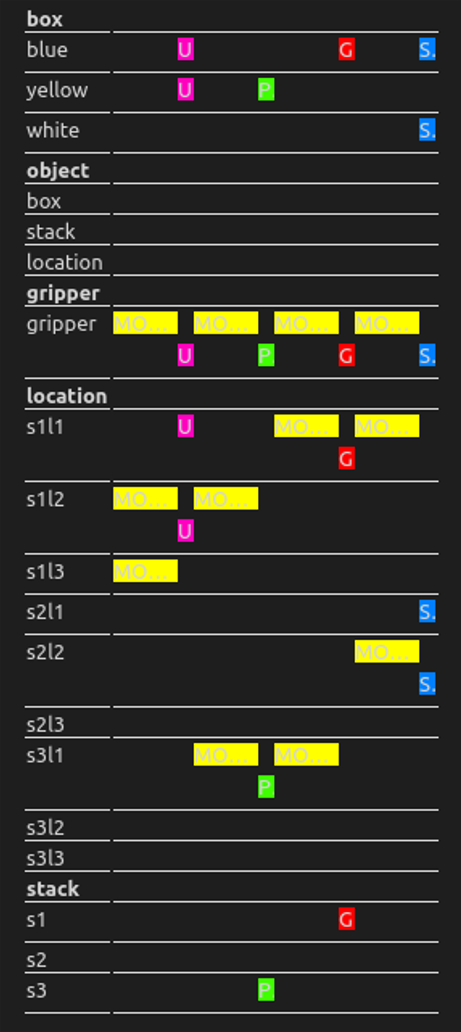
\includegraphics[width=.66\linewidth,keepaspectratio,valign=c]{plugin_vis3}
    \end{minipage}
    \title{Visualisierung eines Plans mit dem PDDL-Plugin}
    \caption{Visualisierung eines Plans mit dem PDDL-Plugin mit Fokus auf die Aktionen (links) und Fokus auf die relevanten Objekte (rechts)}
    \label{fig:pluginvis}
\end{figure}
\subsubsection{Partial Order Planning}{\label{section:pop}}
\emph{\ac{POP}} ist eine Form des Planens, in dem die Aktionen eines Plans nur soweit geordnet sind, wie es notwendig ist \cite{dyer_2003}.
Dies steht im Gegensatz zu \emph{Total-Order} Planern wie \ac{STRIPS}.\\
Es wird nach dem emph{Principle Of Least Commitment} verfahren.
Das bedeutet, dass Entscheidungen soweit wie möglich aufgeschoben und erst getroffen werden, wenn es absolut nötig ist.
Dies umfasst nicht nur die Reihenfolge von Aktionen, sondern auch die Bindung von Variablen.\\
Ein Partial-Order Plan kann als 4-Tupel \cite{grastien} beschrieben werden.
\begin{itemize}
    \item eine Menge von Aktionen
    \item eine Menge von Einschränkungen der Reihenfolge
    \item eine Menge von kausalen Zusammenhängen
    \item eine Menge offener Vorbedingungen (Vorbedingungen einer Aktion, die nicht durch eine andere Aktion erfüllt werden)
\end{itemize}
Die Menge der Aktionen enthält Instanzen von Aktionen der Domäne.
Eine Aktion der Domäne kann daher mehrfach vorkommen.
Einschränkungen der Reihenfolge $A < B$ bilden ab, dass Aktion $A$ vor Aktion $B$ ausgeführt werden muss.
Zyklische Einschränkungen sind nicht erlaubt.
Ein kausaler Zusammenhang $A \xrightarrow{\alpha} B$ beschreibt, dass die Aktion $A$ die Vorbedingung $\alpha$ der Aktion $B$ erfüllt.\\
Die Suche erfolgt im Plan Space.
Jeder Knoten im Graph entspricht einem Teilplan und jede Kante einer Änderung des einen zum anderen Plan.
Dies kann durch das Hinzufügen eines weiteren Schrittes oder einer Einschränkung sowie der Bindung einer Variable geschehen.
Die Wurzel des Graphen besteht aus einem Plan mit zwei Schritten, die den Startzustand und das Ziel darstellen.
Der Startzustand wird durch eine Aktion repräsentiert, die keine Vorbedingungen und alle Fakten als Effekt hat.
Das Ziel erhält alle Zielfakten als Vorbedingung und hat keinen Effekt.
Zusätzlich enthält der Plan die Einschränkung, dass die Aktion für den Start vor der Aktion für das Ziel ausgeführt werden muss ($Start < Ziel$).\\
Ein Plan ist eine Lösung, wenn \cite{grastien}:
\begin{itemize}
    \item keine Aktion des Plans eine offene Vorbedingung hat
    \item und wenn keine Threats existieren
\end{itemize}
Ist der aktuelle Plan keine Lösung, werden folgende Schritte vorgenommen~\cite{grastien}:
\begin{itemize}
    \item eine offene Vorbedingung $p$ einer Aktion $B$ wählen
    \item eine existierende Aktion $A$, die die Vorbedingung $p$ erfüllt wählen oder eine neue Aktion $A$ erzeugen
    \item den kausalen Zusammenhang $A \xrightarrow{p} B$ und die Reihenfolge $A < B$ hinzufügen
    \item wenn $A$ eine neue Aktion ist, die Reihenfolge $Start < A$ hinzufügen
    \item Probleme zwischen dem neuen kausalen Zusammenhang und den existierenden Aktionen lösen sowie zwischen den existierenden kausalen Zusammenhang und $A$, wenn $A$ eine neue Aktion ist.
    \item entsteht durch das Hinzufügen der Reihenfolgen ein Zyklus, kann der Plan keine Lösung mehr werden
\end{itemize}
Ein Problem ist eine Beziehung zwischen einer Aktion $C$ und einem kausalen Zusammenhang  $A \xrightarrow{p} B$, bei der die Aktion $C$ einen Effekt $\neg p$ hat.
Sollte $C$ nach $A$ aber vor $B$ ausgeführt werden, ist die Vorbedingung $p$ für $B$ nicht mehr gegeben.
Probleme können durch \emph{Promotion} oder \emph{Demotion} gelöst werden~\cite{dyer_2003}.
Bei \emph{Promotion} wird der problematische Schritt $C$ nach dem kausalen Zusammenhang ausgeführt: die Reihenfolge $B < C$ wird hinzugefügt.
Bei \emph{Demotion} wird der problematische Schritt $C$ vor dem kausalen Zusammenhang ausgeführt: die Reihenfolge $C < A$ wird hinzugefügt.

\subsubsection{Forward Chaining Partial Order Planning}
Die Prinzipien des \ac{POP} sollen nun mit Vorwärtsverkettung kombiniert werden.
Für Vorwärtsverkettung mit einem Total-Order Plan können Zustände als Tupel $(F,V,Q,P,C)$ beschrieben werden~\citep{popf}:
\begin{itemize}
    \item F ist eine Menge von Fakten, die im Zustand gelten
    \item V enthält die Werte numerischer Variablen
    \item Q ist eine Liste von Aktionen, die begonnen haben, aber noch nicht beendet sind
    \item P ist der Plan, um den Zustand zu erreichen
    \item C ist eine Liste aller zeitlichen Einschränkungen der Schritte in $P$
\end{itemize}
Um eine Aktion zum Plan hinzuzufügen, müssen deren Start- und Endpunkte hinzugefügt werden.
Dies muss nicht in aufeinander folgenden Schritten geschehen.
Wird eine Aktion hinzugefügt werden $F$ und $V$ entsprechend der Effekte angepasst.
Die Voraussetzung, um eine Aktion hinzufügen zu können ist, dass $Q$ keine Aktion enthält, zu der die Effekte der neuen Aktion einen Konflikt darstellen würden.\\
Vorwärtsverkettung im Zustandsraum hat, durch den \emph{Total-Order} Plan, den Vorteil, dass nicht explizit nach Problemen gesucht werden muss.
Neue Aktionen werden immer am Ende hinzugefügt, wodurch sie kein Problem für die Vorbedingungen und Effekte früherer Aktionen darstellen können.
Gleichzeitig kann keine folgende Aktion ein Problem für diese darstellen.
Dieser Vorteil kommt mit dem Nachteil der frühen Bindung und einer festgelegten Reihenfolge zwischen Aktion, zwischen denen kein Zusammenhang besteht.\\
Es soll ein Kompromiss zwischen den Vorteilen von Total- und Partial-Order Planung gefunden werden.
Dem Tupel werden weitere Elemente hinzugefügt:
\begin{itemize}
    \item $F^+(F^-)$, wobei $F^+(p)(F^-(p))$ den Index eines Schrittes $a$ angeben, indem der Fakt $p$ als letztes hinzugefügt (oder gelöscht) wurde
    \item $FP$, wobei $FP(p)$ eine Menge von Paaren $\langle i,d \rangle \in (\mathbb{N}_0 \times \{0,\epsilon\})$:\\
    \begin{itemize}
        \item $\langle i,0 \rangle \in FP(p)$ beschreibt, dass Schritt $i$ am Ende eines offenen Intervalls liegt, in dem $p$ wahr sein muss.\\
        In \ac{PDDL} gibt es diese für Aktionen mit der \emph{over all} Bedingung $p$, wobei $i$ der Endpunkt dieser Aktion ist.
        \item $\langle i,\epsilon \rangle \in FP(p)$ beschreibt, dass Schritt $i$ der Start eines Intervalls ist, indem $p$ wahr sein muss.\\
        Dies entspricht \emph{at start} oder \emph{at end} Bedingungen in \ac{PDDL}, die relevant für den Schritt $i$ sind.
    \end{itemize}
\end{itemize}

\subsubsection{Partial Order Planning Forward}
\ac{POPF} ist ein am King’s College London entwickelter Planer, der die in Abschnitt~\ref{section:pop} genannten Methoden implementiert~\citep{popf}.
Als Heuristik wird ein temporaler \ac{RPG} genutzt.
Ein \ac{RPG} ist ein Planungsgraph, in dem versucht wird, ein vereinfachtes Problem zu lösen.
Die Vereinfachung besteht darin, alle negativen Effekte von Aktionen zu ignorieren.\\
Der Graph besteht aus einer Sequenz $F_0, A_0, ..., F_{t-1}, A_{t-1}, F_t, A_t$: Aktions- und Faktenschichten, die sich abwechseln.
Die Wurzel des Graphen ist eine Faktenschicht, die den aktuellen Zustand abbildet.
Eine Aktionsschicht enthält alle Aktionen, die in der vorhergehenden Faktenschicht anwendbar sind.
Eine Faktenschicht enthält alle Fakten, die durch alle Aktionen der vorhergehenden Aktionsschicht hinzugefügt werden.
Da nur positive Effekte betrachtet werden, enthält eine Faktenschicht auch alle Fakten der vorherigen Faktenschicht und eine Aktionsschicht ebenfalls alle Aktionen der vorherigen Aktionsschicht.\\
Ein Beispiel eines \ac{RPG} ist in Abbildung~\ref{fig:rpg} dargestellt.
Im Startzustand gelten die Fakten $at(Home)$ und $has(Money)$, dargestellt in $F_0$.
Die einzige Aktion, deren Vorbedingungen erfüllt ist, ist $move(Home, Shop)$ und wird der Aktionsschicht $A_0$ hinzugefügt.
Pfeile, die zu Aktionen gehen, zeigen die Fakten, die als Vorbedingung gelten.
Pfeile, die zu Fakten gehen, zeigen die Aktionen, durch deren Effekt sie hinzugefügt wurden.
In $F_1$ wird als Effekt der Aktion $move(Home, Shop)$ der Fakt $at(Shop)$ hinzugefügt.
Da negative Effekte ignoriert werden, gilt $at(Home)$ weiterhin.
Da in $F_1$ nun $at(Shop)$ und $has(Money)$ gelten, kann in $A_1$ die Aktion $buy(Product, Money)$ angewendet werden.
Dies resultiert in dem Fakt $has(Product)$ in $F_2$.\\
Angenommen, das Ziel ist $has(Product)$, so ist dieses Ziel in $F_2$ erfüllt.
Mit $t = 2$ als Wert der Heuristik, wird gezeigt, dass mindestens zwei Aktionen nötig sind um vom Startzustand zum Ziel zu gelangen.
Da $at(Home)$ vom Startzustand aus durchgängig gilt, erhält jedoch auch das Ziel $\{at(Home),has(Product)\}$ den Heuristikwert 2.\\
\begin{figure}[ht!]
    \centering
    \tikzset{every picture/.style={line width=0.75pt}} %set default line width to 0.75pt

    \begin{tikzpicture}[x=0.75pt,y=0.75pt,yscale=-1,xscale=1]
%uncomment if require: \path (0,355); %set diagram left start at 0, and has height of 355

%Shape: Rectangle [id:dp564712349225938]
        \draw  [fill={rgb, 255:red, 228; green, 250; blue, 206 }  ,fill opacity=1 ] (104,8) -- (546,8) -- (546,48) -- (104,48) -- cycle ;
%Rounded Rect [id:dp5993299884546457]
        \draw   (101,88) .. controls (101,83.58) and (104.58,80) .. (109,80) -- (540,80) .. controls (544.42,80) and (548,83.58) .. (548,88) -- (548,112) .. controls (548,116.42) and (544.42,120) .. (540,120) -- (109,120) .. controls (104.58,120) and (101,116.42) .. (101,112) -- cycle ;
%Shape: Rectangle [id:dp4448475604191735]
        \draw  [fill={rgb, 255:red, 228; green, 250; blue, 206 }  ,fill opacity=1 ] (105,152) -- (547,152) -- (547,192) -- (105,192) -- cycle ;
%Rounded Rect [id:dp06633752127787629]
        \draw   (102,228) .. controls (102,223.58) and (105.58,220) .. (110,220) -- (541,220) .. controls (545.42,220) and (549,223.58) .. (549,228) -- (549,252) .. controls (549,256.42) and (545.42,260) .. (541,260) -- (110,260) .. controls (105.58,260) and (102,256.42) .. (102,252) -- cycle ;
%Shape: Rectangle [id:dp8200443828072568]
        \draw  [fill={rgb, 255:red, 228; green, 250; blue, 206 }  ,fill opacity=1 ] (104,290) -- (546,290) -- (546,330) -- (104,330) -- cycle ;

% Text Node
        \draw (184,17) node [anchor=north west][inner sep=0.75pt]   [align=left] {at(Home)};
% Text Node
        \draw (255,90) node [anchor=north west][inner sep=0.75pt]   [align=left] {move(Home, Shop)};
% Text Node
        \draw (189,160) node [anchor=north west][inner sep=0.75pt]   [align=left] {at(Home)};
% Text Node
        \draw (329,160) node [anchor=north west][inner sep=0.75pt]   [align=left] {at(Shop)};
% Text Node
        \draw (115,230) node [anchor=north west][inner sep=0.75pt]   [align=left] {move(Home, Shop)};
% Text Node
        \draw (394,17) node [anchor=north west][inner sep=0.75pt]   [align=left] {has(Money)};
% Text Node
        \draw (450,160) node [anchor=north west][inner sep=0.75pt]   [align=left] {has(Money)};
% Text Node
        \draw (399,230) node [anchor=north west][inner sep=0.75pt]   [align=left] {buy(Product, Money)};
% Text Node
        \draw (119,300) node [anchor=north west][inner sep=0.75pt]   [align=left] {at(Home)};
% Text Node
        \draw (361,300) node [anchor=north west][inner sep=0.75pt]   [align=left] {at(Shop)};
% Text Node
        \draw (233,300) node [anchor=north west][inner sep=0.75pt]   [align=left] {has(Money)};
% Text Node
        \draw (447,300) node [anchor=north west][inner sep=0.75pt]   [align=left] {has(Product)};
% Text Node
        \draw (258,230) node [anchor=north west][inner sep=0.75pt]   [align=left] {move(Shop, Home)};
% Text Node
        \draw (30,20.4) node [anchor=north west][inner sep=0.75pt]    {$F_{0}$};
% Text Node
        \draw (30,93.4) node [anchor=north west][inner sep=0.75pt]    {$A_{0}$};
% Text Node
        \draw (30,160) node [anchor=north west][inner sep=0.75pt]    {$F_{1}$};
% Text Node
        \draw (30,230) node [anchor=north west][inner sep=0.75pt]    {$A_{1}$};
% Text Node
        \draw (30,300) node [anchor=north west][inner sep=0.75pt]    {$F_{2}$};
% Connection
        \draw    (234.39,38) -- (301.47,84.85) ;
        \draw [shift={(303.11,86)}, rotate = 214.94] [color={rgb, 255:red, 0; green, 0; blue, 0 }  ][line width=0.75]    (10.93,-3.29) .. controls (6.95,-1.4) and (3.31,-0.3) .. (0,0) .. controls (3.31,0.3) and (6.95,1.4) .. (10.93,3.29)   ;
% Connection
        \draw    (327.69,111) -- (351.37,155.24) ;
        \draw [shift={(352.31,157)}, rotate = 241.84] [color={rgb, 255:red, 0; green, 0; blue, 0 }  ][line width=0.75]    (10.93,-3.29) .. controls (6.95,-1.4) and (3.31,-0.3) .. (0,0) .. controls (3.31,0.3) and (6.95,1.4) .. (10.93,3.29)   ;
% Connection
        \draw    (486.7,184) -- (473.89,226.09) ;
        \draw [shift={(473.3,228)}, rotate = 286.93] [color={rgb, 255:red, 0; green, 0; blue, 0 }  ][line width=0.75]    (10.93,-3.29) .. controls (6.95,-1.4) and (3.31,-0.3) .. (0,0) .. controls (3.31,0.3) and (6.95,1.4) .. (10.93,3.29)   ;
% Connection
        \draw    (378.45,182) -- (448.36,226.92) ;
        \draw [shift={(450.05,228)}, rotate = 212.72] [color={rgb, 255:red, 0; green, 0; blue, 0 }  ][line width=0.75]    (10.93,-3.29) .. controls (6.95,-1.4) and (3.31,-0.3) .. (0,0) .. controls (3.31,0.3) and (6.95,1.4) .. (10.93,3.29)   ;
% Connection
        \draw    (473.29,253) -- (486.64,297.09) ;
        \draw [shift={(487.21,299)}, rotate = 253.15] [color={rgb, 255:red, 0; green, 0; blue, 0 }  ][line width=0.75]    (10.93,-3.29) .. controls (6.95,-1.4) and (3.31,-0.3) .. (0,0) .. controls (3.31,0.3) and (6.95,1.4) .. (10.93,3.29)   ;
% Connection
        \draw    (352.66,182) -- (331.25,224.22) ;
        \draw [shift={(330.34,226)}, rotate = 296.9] [color={rgb, 255:red, 0; green, 0; blue, 0 }  ][line width=0.75]    (10.93,-3.29) .. controls (6.95,-1.4) and (3.31,-0.3) .. (0,0) .. controls (3.31,0.3) and (6.95,1.4) .. (10.93,3.29)   ;

    \end{tikzpicture}
    \caption{\ac{RPG} für das Ziel $\{at(Home), has(Product)\}$}
    \label{fig:rpg}
\end{figure}
Die Erstellung des Graphen wird gestoppt, wenn eine Faktenschicht alle Ziele erfüllt oder wenn eine Faktenschicht der vorherigen entspricht.
Werden zwischen zwei Faktenschichten keine neuen Fakten hinzugefügt, können auch in zukünftigen Faktenschichten keine neuen Fakten mehr hinzugefügt werden.
Endet ein Graph auf diese Weise, ist das vereinfachte Problem nicht lösbar und der Zustand erhält einen Heuristikwert von \emph{unendlich}.
Andernfalls wird ein vereinfachter Plan aus dem Graphen extrahiert.
Die Länge des optimalen vereinfachten Plans ist eine zulässige Heuristik.
Der optimale Plan lässt sich jedoch nicht effizient extrahieren~\cite{hoffmannnebel2001}.
Daher wird ein suboptimaler Plan extrahiert, wodurch die Heuristik nicht mehr zulässig ist.\\
Um einen \ac{RPG} für temporales Planen zu erweitern, werden Aktionen in Startaktionen $A_\vdash$ und Endaktionen $A_\dashv$ aufgeteilt, die jeweils nur \emph{at start} und \emph{at end} Effekte enthalten.
Der Index $t$ einer Schicht entspricht nun einem Zeitstempel.\\
Als Suchverfahren wird zunächst \ac{EHC} versucht.
Der in Abbildung~\ref{fig:ehc_algo} beschriebene Algorithmus beginnt im Startzustand $S$.
\begin{figure}[h!]
           \centering
           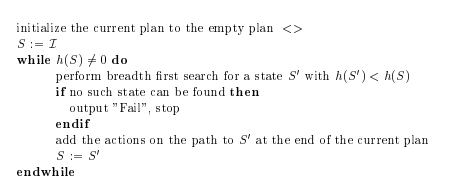
\includegraphics{ehc_algo}
           \caption{\ac{EHC} Algorithmus~\cite{hoffmannnebel2001}}
           \label{fig:ehc_algo}
\end{figure}
Von diesem aus wird wird eine \emph{breadth-first} Suche gestartet.
Diese findet den nächstbesten Nachfolger, also den nächsten Zustand $S'$, dessen Heuristik besser als die des aktuellen Zustands ist.
Gelingt dies, wird der Weg von $S$ nach $S'$ zum Plan hinzugefügt.
Die Suche wird gestoppt, wenn ein Zustand mit der Heuristik 0 gefunden wird.
Ist die Heuristik des aktuellen Zustands $\neq 0$ und wird kein Zustand mit einer besseren Heuristik gefunden, schlägt der Algorithmus fehl.
Zustände werden in einer \emph{Queue} gespeichert und für eine Iteration der Suche wird der erste Zustand $S'$ von dieser entfernt und und die Heuristik berechnet.
Die Suche ist erfolgreich, wenn die Heuristik für diesen Zustand $S'$ besser als die von $S$ ist.
Andernfalls werden die Nachfolger von $S'$ zum Ende der \emph{Queue} hinzugefügt.
Wiederholte Zustände werden durch ein \emph{HashTable} der bereits besuchten Zustände vermieden.
Die Suche schlägt fehl, wenn keine weiteren Zustände erreicht werden können.\\
Wird in einer Iteration kein besserer Zustand gefunden, stoppt \ac{EHC}, ohne eine Lösung zu finden.
Dies geschieht, da \ac{EHC} Entscheidungen, eine Aktion in den Plan aufzunehmen, nie rückgängig macht.
Der Algorithmus ist daher nur vollständig für Planungsaufgaben, die keine \emph{"dead ends"} enthalten.
Ein \emph{Dead End} für eine Planungsaufgabe $(O,I,G)$ ist definiert als ein Zustand $S$, der erreichbar ist und von diesem aus keine Plan das Ziel erreichen kann:\\
$\exists P: S = Result(I,P)$  und  $\neg\exists P': G\subseteq Result(S,P')$\\
Schlägt die Suche mit \ac{EHC} fehl, wird eine neue \emph{best-first} Suche ausgehend vom ursprünglichen Startzustand gestartet.
\subsubsection{Behavior Tree}
\acp{BT} sind ein modulares System, das in der Videospieleindustrie entwickelt wurde~\cite{bt_book}.
Sie ermöglichen aus simplen Aktionen komplexe Verhaltensmuster zu modelieren ohne das Aktionen Kenntnis über andere Aktionen haben müssen~\cite{bt_robotics}.
Entsprechend~\cite{bt_1} ist ein \ac{BT} ein gerichteter azyklischer Graph $G(V,E)$ mit $|V|$ Knoten und $|E|$ Kanten.
Ein Elternknoten von einem Paar verbundener Knoten ist der, von dem die Kante ausgeht.
Der Knoten mit der eingehenden Kante ist ein Kindknoten.
Knoten ohne Kinder heißen Blätter.
Ein Knoten ohne Eltern heißt Wurzel.
In einem \ac{BT} gibt es genau eine Wurzel mit genau einem Kind.\\
Nach~\cite{bt_book} beginnt die Ausführung eines \ac{BT} bei der Wurzel, die in einem bestimmten Intervall ein Signal erzeugt, dass die Ausführung eines Knoten erlaubt (''tick'').
Dieses Signal wird an das Kind der Wurzel gesendet.
Ein Knoten wird ausgeführt, wenn es dieses Signal erhält und auch nur dann.
Wird ein Knoten ausgeführt, gibt er einen Status zurück.
Der Status ist einer von drei möglichen~\cite{bt_uav}:
\begin{itemize}
    \item Running: die Ausführung läuft noch
    \item Success: die Ausführung war erfolgreich
    \item Failure: die Ausführung ist fehlgeschlagen
\end{itemize}\\
Wie in~\cite{bt_1} beschrieben, werden verschiedene Arten von Knoten auf verschiedene Typen beschränkt.
Blätter sind Ausführungsknoten und haben einen der folgenden Typen:
\begin{itemize}
    \item Aktion
    \item Bedingung
\end{itemize}
Knoten mit Kindern, mit Ausnahme der Wurzel, sind Kontrollflussknoten und haben einen der folgenden Typen:
\begin{itemize}
    \item Selektor
    \item Sequenz
    \item Parallel
    \item Dekorator
\end{itemize}
Ein Selektor-Knoten führt seine Kinder der Reihe nach aus, bis das erste einen Status \emph{Running} oder \emph{Success} zurückgibt.
Nachfolgende Kinder werden dann nicht mehr ausgeführt und der Selektor gibt den entsprechenden Status zurück.
Wurden alle Kinder ausgeführt und keins hat einen Status \emph{Running} oder \emph{Success} zurückgegeben, gibt der Selektor den Status \emph{Failure} zurück.\\
Ein Sequenz-Knoten führt seine Kinder der Reihe nach aus, bis das erste einen Status \emph{Running} oder \emph{Failure} zurückgibt.
Nachfolgende Kinder werden dann nicht mehr ausgeführt und die Sequenz gibt den entsprechenden Status zurück.
Wurden alle Kinder ausgeführt und keins hat einen Status \emph{Running} oder \emph{Failure} zurückgegeben, gibt die Sequenz den Status \emph{Success} zurück.\\
Ein Parallel-Knoten führt alle Kinder aus, ohne auf den Status des vorherigen zu warten.
Überschreitet die Anzahl der Kinder, die \emph{Success} zurückgeben einen benutzerdefinierten Wert $S$, gibt der Knoten \emph{Success} zurück.
Haben $N-M+1$ Kinder \emph{Failure} zurückgegeben, wobei $N$ die Anzahl der Kinder ist, wird \emph{Failure} zurückgeben, da der Wert $S$ nicht mehr erreicht werden kann~\cite{bt_book}.
Alternativ kann ein zweiter benutzerdefinierter Wert $F$ eingeführt werden.
Überschreitet die Anzahl der Kinder, die \emph{Failure} zurückgeben diesen Wert $F$, wird direkt \emph{Failure} zurückgegeben~\cite{bt_1}.
$S$ und $F$ müssen $\leq M$ sein.
Wird keiner dieser beiden Werte überschritten, wird \emph{Running} zurückgegeben.\\
Ein Dekorator-Knoten hat genau ein Kind.
Er kann durch eine Bedingung entscheiden, ob das Kind ausgeführt wird und kann einen modifizierten Status zurückgeben.
Beispiele für Dekoratoren sind:
\begin{itemize}
    \item Invertierung/Negation: der \emph{Success} und \emph{Failure} Status des Kinds wird invertiert
    \item Zeitbeschränkung: gibt das Kind den Status \emph{Running} für länger als eine benutzerdefinierter Zeitspanne $T$ zurück, wird \emph{Failure} zurückgegeben und das Kind nicht mehr ausgeführt
\end{itemize}\cite{bt_book}

\begin{table}[]
    \resizebox{\textwidth}{!}{%
        \begin{tabular}{|l|l|lll|}
            \hline
            \multicolumn{1}{|c|}{\multirow{2}{*}{\textbf{Knoten}}} &
            \multirow{2}{*}{\textbf{Symbol}} &
            \multicolumn{3}{c|}{\textbf{Rückgabewert}} \\ \cline{3-5}
            \multicolumn{1}{|c|}{} &
            &
            \multicolumn{1}{l|}{\textbf{Success}} &
            \multicolumn{1}{l|}{\textbf{Failure}} &
            \textbf{Running} \\ \hline
            Selektor &
            &
            \multicolumn{1}{l|}{\begin{tabular}[c]{@{}l@{}}Wenn 1 Kind ''Success'' \\ zurückgibt\end{tabular}} &
            \multicolumn{1}{l|}{\begin{tabular}[c]{@{}l@{}}Wenn alle Kinder ''Failure''\\ zurückgeben\end{tabular}} &
            \begin{tabular}[c]{@{}l@{}}Wenn 1 Kind ''Running''\\ zurückgibt\end{tabular} \\ \hline
            Sequenz &
            &
            \multicolumn{1}{l|}{\begin{tabular}[c]{@{}l@{}}Wenn alle Kinder ''Success''\\  zurückgeben\end{tabular}} &
            \multicolumn{1}{l|}{\begin{tabular}[c]{@{}l@{}}Wenn 1 Kind ''Failure''\\ zurückgibt\end{tabular}} &
            \begin{tabular}[c]{@{}l@{}}Wenn 1 Kind ''Running''\\ zurückgibt\end{tabular} \\ \hline
            Parallel &
            &
            \multicolumn{1}{l|}{\begin{tabular}[c]{@{}l@{}}Wenn $\geq M$ Kinder ''Success''\\  zurückgeben\end{tabular}} &
            \multicolumn{1}{l|}{\begin{tabular}[c]{@{}l@{}}Wenn $> N - M$ Kinder ''Failure''\\ zurückgeben\end{tabular}} &
            \begin{tabular}[c]{@{}l@{}}Wenn keine der Bedingungen\\  für ''Success'' oder ''Failure'' \\ erfüllt sind\end{tabular} \\ \hline
            Dekorator &
            &
            \multicolumn{1}{l|}{benutzerdefiniert} &
            \multicolumn{1}{l|}{benutzerdefiniert} &
            benutzerdefiniert \\ \hline
            Bedingung &
            &
            \multicolumn{1}{l|}{Wenn wahr} &
            \multicolumn{1}{l|}{Wenn falsch} &
            Nie \\ \hline
            Aktion &
            &
            \multicolumn{1}{l|}{Bei vollständiger Ausführung} &
            \multicolumn{1}{l|}{\begin{tabular}[c]{@{}l@{}}Wenn vollständige Ausführung\\ nicht möglich ist\end{tabular}} &
            Während der Ausführung \\ \hline
        \end{tabular}%
    }
    \caption{Übersicht der \ac{BT} Knoten, nach~\cite{bt_book}}
    \label{tab:btoverview}
\end{table}
- Visualisierungs bsp.\\
\subsection{Planung in \ac{ROS2}}
Für die Planung in \ac{ROS2} wird \ac{PlanSys2} genutzt.
In diesem Abschnitt wird das in~\cite{plansys} beschriebene System zusammenfassend beschrieben.
Es wird dabei jedoch nur auf die für diese Arbeit relevanten Teile eingegangen.\\
\ac{PlanSys2} ist ein modulares OpenSource Planungsframework.
Ursprünglich als Nachfolger für ROSPlan~\cite{rosplan} geplant, bietet es viel umfangreichere Funktionen.
Hierfür werden unter anderem neue Funktionen von \ac{ROS2} wie LifeCycle-Knoten oder Multicast Kommunikation genutzt.\\
Eins der Designprinzipien bei der Entwicklung von \ac{PlanSys2} ist Modularität und Erweiterbarkeit.
Alle Komponenten haben klar definierte Schnittstellen, wodurch sie einfach erweitert oder ausgetauscht werden können.\\
Die Hauptkomponente ist der \emph{''Planner''} Knoten, der den tatsächlichen Planer aufruft.
Verschiedene Planer können über Plugins aufgerufen werden, die beschreiben, wie der Planer aufzurufen ist und wie der generierte Plan zu verstehen ist.
Standardmäßig sind \ac{POPF} sowie TFD (\emph{Temporal Fast Downward})~\cite{tfd} verfügbar und konfiguriert.\\
Der \emph{''Domain Expert''} Knoten liest die Domäne im \ac{PDDL}-Format ein.
Er kann mehrere verschiedene Domänen zu einer kombinieren.
Dies ermöglicht es, mehrere modulare Packages zu nutzen, die jeweils nur den für sie relevanten Teil einer Domäne beinhalten sowie deren Aktionen  implementieren.
Der Knoten dient zur Validierung (z.B. ob ein Prädikat, das hinzugefügt werden soll, mit den gegeben Objekten gültig ist) und dem Planer die Domäne zur Verfügung zu stellen.\\
Der \emph{''Problem Expert''} Knoten enthält alle Informationen zum gegebenen Problem: Objekte, Prädikate, Funktionen und Ziele.
Diese werden immer über den \emph{''Domain Expert''} validiert.
Wenn ein Plan angefordert wird, werden die gespeicherten Informationen zu einem Problem im \ac{PDDL} Format konvertiert und dem \emph{''Planner''} Knoten zur Verfügung gestellt.\\
Der \emph{''Executor''} Knoten ist dafür zuständig einen generierten Plan auszuführen.
Der Plan wird in einen \ac{BT} konvertiert, der diesen ausführt.\\
Ein weiteres Konzept ist die Unterstützung für mehrere Roboter sowie eine Spezialisierung bei der Ausführung von Aktionen.
Alle Knoten im gleichen Netzwerk können miteinander kommunizieren.
Es kann mehrere Knoten geben, die die gleiche Domänenaktion ausführen, sich aber auf bestimmte Parameter spezialisieren.
Mehrere Roboter können einen Knoten für die gleiche Aktion \emph{(move roboter start ziel)} ausführen, wobei sich jede darauf spezialisiert, die Aktion auszuführen, deren erster Parameter mit dem entsprechenden Roboter übereinstimmt.
Die gleiche Aktion kann je nach vorhandenen Parametern von verschiedenen Knoten ausgeführt werden.\\
\acp{BT} eignen sich für die Ausführung eines Plans, da sich mit ihnen sehr gut sequentielle und parallele Vorgänge beschreiben lassen.
Zunächst wird von einem Plan ein Ausführungs-Graph erstellt, der die Abhängigkeiten zwischen Aktionen zeigt.
Von diesen lässt sich ableiten, welche Aktionen parallel ausgeführt werden können und welche sequentiell ausgeführt werden müssen.
Semantisch entspricht jedes Blatt im Graphen einer Aktion.
In der Praxis ist jedes Blatt ein eigenständiger \ac{BT}, der nicht nur die selbst Aktion ausführt, sondern auch die Bedingungen überprüft und die Effekte ausführt (s. Abbildung~\ref{fig:plansysbtaction}).\\
\begin{figure}
    \centering
    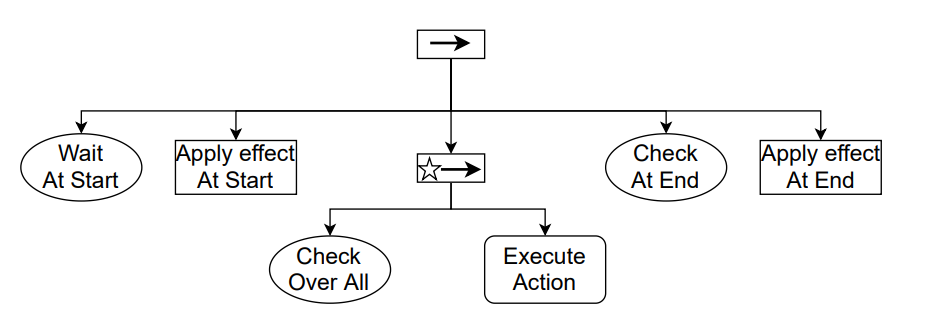
\includegraphics[width=\textwidth]{plansys2btaction}
    \caption{\ac{BT} zur Ausführung einer spezifischen Aktion~\cite{plansys}}
    \label{fig:plansysbtaction}
    \end{figure}
\ac{PlanSys2} hat drei große Limitationen.
\ac{PDDL}-Unterstützung beschränkt sich aktuell auf \ac{PDDL} 2.1 mit dem Ziel zukünftig, die aktuellste Version zu unterstützen.
Wird eine Aktion und damit ein Plan abgebrochen, gibt es keine Garantie, dass der Zustand der Welt konsistent bleibt.
Die Fähigkeit von Planern, die zunächst einen allgemeinen Plan liefern und diesen während der Ausführung verbessern, wird nicht genutzt.
Eine geplante Funktion ist jedoch, Übergänge von der Ausführunge eines Plans zu einem anderen zu ermöglichen.
labe\section{Konzept}{\label{konzept}}
In diesem Abschnitt wird der Ansatz beschrieben, mit dem in dieser Arbeit vorgegangen werden soll.
\subsection{Inbetriebnahme}
Im ersten Schritt muss der OMX in Betrieb genommen werden. Dies beinhaltet den Zusammenbau und Konfiguration sowie die Installation nötiger Software. Ein besonderes Augenmerk wird dabei darauf gelegt,  Details festzuhalten welche in den gegebenen Anleitungen nicht explizit angegeben werden oder leicht zu übersehen sind.
\subsection{Struktur Nodes}{\label{konzept:nodes}}
Um eine einfache sowie übersichtliche Steuerung des Greifarms zu ermöglichen wird die Funktionalität in mehrere ROS2 Nodes aufgeteilt. Generell werden folgende Funktionalitäten benötigt: der Planer, die Speicherung des aktuellen Zustands der Welt, die Ausführung des Plans sowie die Möglichkeit Eingaben zu verarbeiten und an die entsprechenden Nodes weiterzuleiten.\\
Diese Aufteilung entspricht auch einer guten Aufteilung und Trennung der Verantwortungen um daraus ROS2 Nodes zu machen. Hier haben die Nodes folgende Verantwortlichkeiten:\\
Die Planungs-Node muss mit einer gegebenen Domäne und einem Problem einen Plan bestehend aus einer Reihe von Aktionen zurückgeben.\\
Die Welt-Node hält den aktuellen Zustand der Welt bzw. des Problems und muss diesen konsistent halten.\\
Die Ausführungs-Node muss entsprechend eines Plans die gegeben Aktionen ausführen.\\
Die Eingabe-Node ermöglicht die Erstellung eines Problems mit einem Welt-Zustand und einem Ziel.
\subsection{Planungsmodell}{\label{konzept:planningmodel}}
Für die Erstellung von Plänen wird eine Domäne im \ac{PDDL} Format erstellt. In der Domäne werden die Aspekte des Stapelns von Blöcken mit denen des Greifers kombiniert. Zusätzlich werden \emph{durative actions} genutzt um die Dauer der einzelnen Aktionen zu modellieren.
\subsection{Erstellung von Übungsbeispielen}{\label{konzept:exercise}}
Abschließend soll eine Übersicht, mit Möglichkeiten den OMX in die Lehre einzubinden,  erstellt werden. Dies umfasst spezifische Beispiele sowie allgemeine Ansatzpunkte um die Benutzung des OMX sowie dessen grundlegenden Konzepte zu vermitteln.
\section{Implementierung}

\subsection {Inbetriebnahme Greifarm}
Der OMX wird als Bausatz geliefert.
Für die Inbetriebnahme ist daher der Zusammenbau und die Installation der entsprechenden Software nötig.
\subsubsection{Zusammenbau}
Der Bausatz des OMX besteht aus ca.\ 60 Teilen (ohne Schrauben, s.\ Abbildung~\ref{fig:omxparts}).Einige der mit den Servomotoren mitgelieferten Teile werden dabei nicht benötigt, da der Bausatz des OMX diese auch enthält oder ersetzt (z.B.\ längere Kabel).
Von allen Schrauben wurde außerdem Ersatz mitgeliefert.\\
Der Zusammenbau erfolgte nach der auf der Webseite verfügbaren Bauanleitung VERWEIS ANLEITUNG. Zu beachten ist, dass hier vorausgesetzt wird, dass den Servos bereits die IDs 11 (Basis des Greifarms) bis 15 (Greifer) zugewiesen wurden.
Dies kann über die Software DYNAMIXEL Wizard{\footnote{VERWEIS ODER LINK}} gemacht werden: die Servos einzeln über das U2D2 (s. Abschnitt {\ref{u2d2}}) an den PC anschließen, die ID setzen und den Servo entsprechend markieren oder die ID merken.
Weiterhin müssen bei den Abdeckungen der Servos 12 und 14 die vorgestanzten Abdeckungen herausgebrochen werden.
Dies ist in der Anleitung leicht zu übersehen.
Weiterhin wird angenommen, dass das Horn der Servos bereits angebracht ist.
Hierbei ist darauf zu achten, dass die Einkerbung an Horn und Servo übereinstimmen.
\begin{figure}[ht!]
\centering
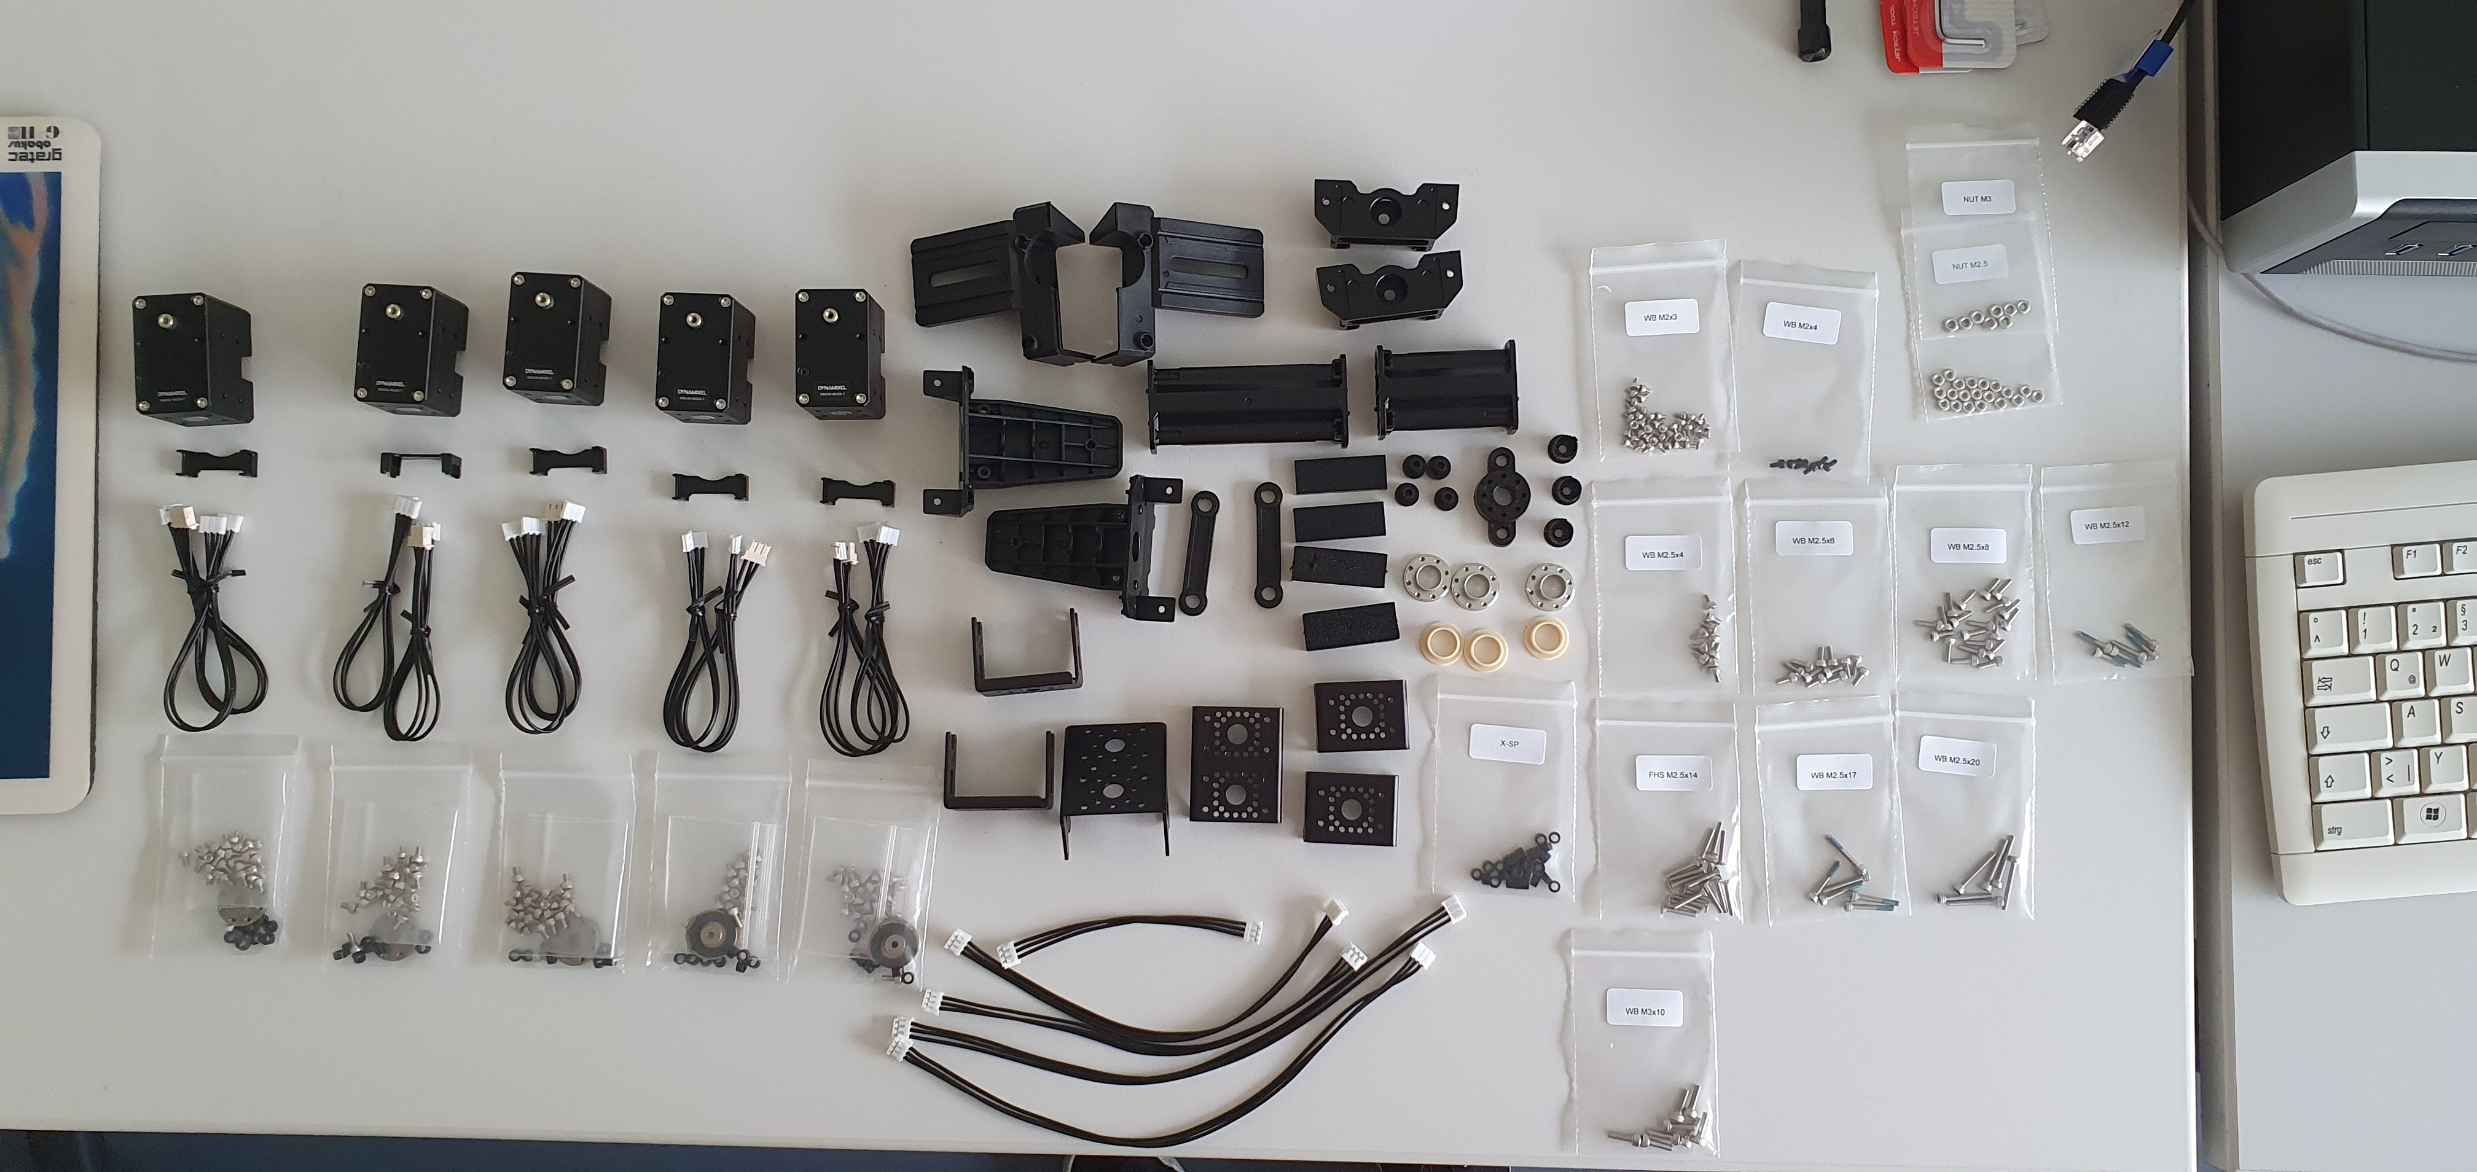
\includegraphics[width=\textwidth]{parts}
\caption{Bausatz für den OpenMANIPULATOR-X}
\label{fig:omxparts}
\end{figure}
\subsubsection{Virtuelle Maschine}
Zur Nutzung des Greifarms wurde eine \ac{VM} mit VirtualBox {\footnote{https://www.virtualbox.org}} von Oracle aufgesetzt.
Als Betriebssystem der \ac{VM} wurde das für ROS2 Foxy empfohlene~\citep{foxyreq} Ubuntu 20.04 {\footnote{\url{https://releases.ubuntu.com/20.04/}}} gewählt.
Danach wurde entsprechend der Anleitung für den OpenMANIPULATOR-X~\citep{foxyinstall} zuerst ROS 2 Foxy über das Installations-Script von ROBOTIS und im Anschluss die für den Greifarm benötigten Packages installiert.

\subsection{Steuerung OMX}
Die Steuerung des OMX erfolgt über die vom \emph{open\_manipulator\_x\_controller}\\ \verb|open_manipulator_x_controller| zur Verfügung gestellten Topics und Services.

\subsubsection{Anschluss über U2D2}{\label{u2d2}}
Der OMX wird über das U2D2 und das U2D2 Power Hub Board (s. Abbildung~\ref{fig:u2d2}) per USB an den PC angeschlossen.\\
Das U2D2 konvertiert die Signale der DYNAMIXEL und ermöglicht die Kontrolle über den PC. Zur Nutzung des U2D2 in der \ac{VM} muss das Gerät \emph{FTDI USB <-> Serial Converter} über das Geräte-Menü der \ac{VM} an diese gebunden werden (s. Abbildung~\ref{fig:ftdivm}).
\begin{figure}[ht!]
\centering
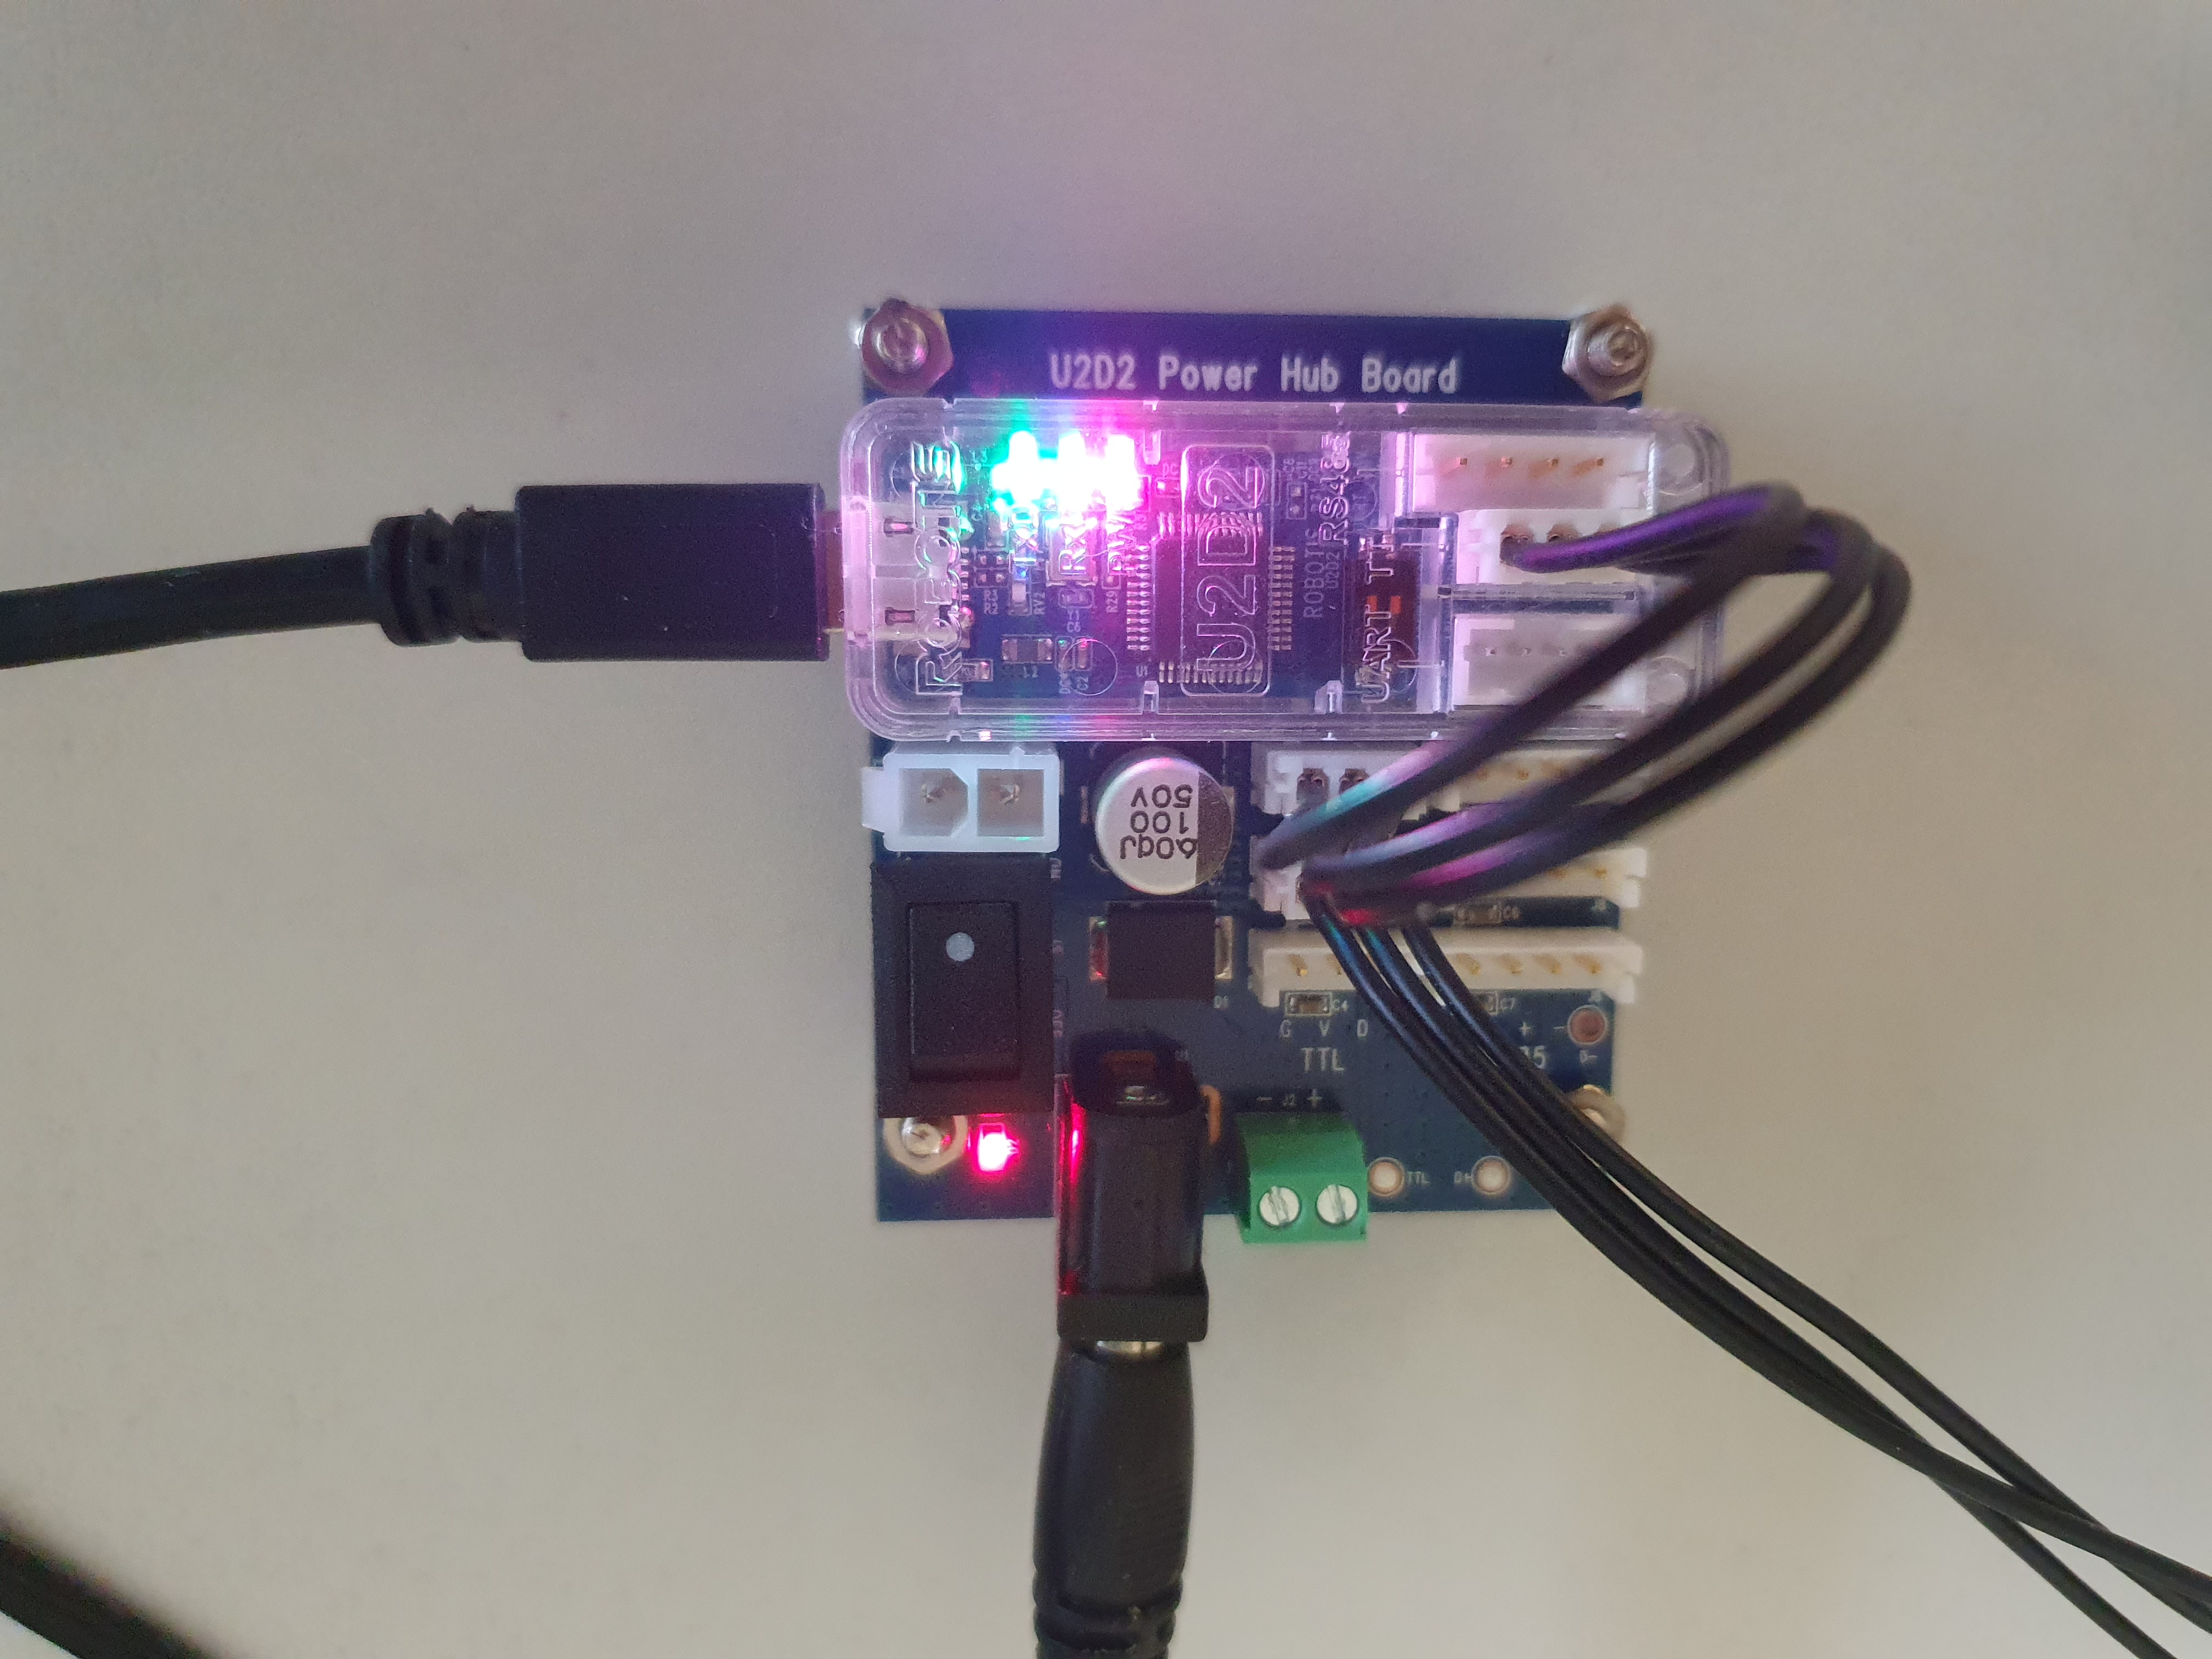
\includegraphics[width=\textwidth]{u2d2}
\caption{U2D2 Power Hub Board mit montiertem U2D2 (rechts im Bild)}
\label{fig:u2d2}
\end{figure}
\begin{figure}[ht!]
\centering

\includegraphics[width=\textwidth]{ftdivm}
\caption{Geräte-Menü der \ac{VM} mit angeschlossenem U2D2}
\label{fig:ftdivm}
\end{figure}


\subsubsection{OMX-Controller}
Der OMX-Controller ist ein Package, welches automatisch beim Installieren der für den OMX benötigten Software installiert wird.
Er kann über die entsprechende Launch-Datei mit dem Befehl
\begin{verbatim}
ros2 launch open_manipulator_x_controller 
     open_manipulator_x_controller.launch.py
\end{verbatim}
gestartet werden.
\subsubsection{Joint und Task Space}
Der OMX kann in den zwei verschiedenen Arbeitsräumen \emph{Joint Space} und \emph{Task Space} betrachtet werden.\\
Im \emph{Joint Space} werden die Gelenke und ihre aktuellen Winkel betrachtet.\\
Der \emph{Task Space} entspricht einer Betrachtung in einem kartesischen Koordinatensystem, mit dem Motor mit der ID 11 als Ursprung.
Zusätzlich zur Position gibt es eine Orientierung für jede Achse (Roll-Nick-Gier, engl.\ roll-pitch-yaw).
\subsubsection{Topics}
Der OMX-Controller veröffentlicht drei Topics, die Informationen über den aktuellen Status geben:
\begin{itemize}
    \item /states
    \item /joint\_states
    \item /kinematics\_pose
\end{itemize}
\emph{/states} stellt allgemeine Informationen über die Motoren und die Bewegung des OMX zur Verfügung.
Ob die Motoren aktiviert sind, wird über das Feld \emph{open\_manipulator\_actuator\_state} mit den möglichen Werten \emph{ACTUATOR\_ENABLE} und \emph{ACTUATOR\_DISABLE} angegeben.
Der Bewegungsstatus, mit den möglichen Werten \emph{IS\_MOVING} und \emph{STOPPED}, steht im Feld \emph{open\_manipulator\_moving\_state}.\\
\emph{/joint\_states} stellt Informationen über alle Gelenke zur Verfügung.
Dies umfasst den Namen, den aktuell verbrauchten Strom, die Position (der Winkel des Motors) sowie die Geschwindigkeit.\\
\emph{/kinematics\_pose} stellt Informationen über die Pose im Task Space zur Verfügung.
Eine Pose besteht dabei aus einer Position und einer Orientierung und bezieht sich auf den Greifer.
Die Position enthält die Koordinaten der Mitte des Greifers.
Die Orientierung gibt die Rotation als Quaternion an.

\subsubsection{Kinematik}
Der OMX lässt sich über zwei Formen der Kinematik steuern.
Zum eine über die direkte Kinematik (auch Vorwärtskinematik, engl.\ forward kinematics, FK), was einer Steuerung im Joint Space entspricht und zum anderen über die inverse Kinematik (engl.\ inverse kinematics, IK), was einer Steuerung im Task Space entspricht.\\
Die komplette kinematische Steuerung erfolgt über Services, die sich dementsprechend darin unterscheiden, ob Winkel für die Gelenke oder Posen für den Greifer angegeben werden.
Bei der Steuerung über Posen besteht wiederum die Möglichkeit Position und Orientierung oder nur eines der beiden zu steuern und den aktuellen Wert des anderen beizubehalten.\\
Die komplette Liste der Services ist in der Anleitung des OMX\footnote{\url{https://emanual.robotis.com/docs/en/platform/openmanipulator_x/ros_controller_msg/#message-list}} zu finden.


\subsubsection{Teleop} \label{teleop}
Mit einem laufenden OMX-Controller kann der OMX auch ohne extra Programmierung direkt ferngesteuert werden.
Mögliche Geräte zur Steuerung sind die Tastatur sowie Playstation- und XBOX-Controller.
Für \ac{ROS2} Foxy wird aktuell allerdings nur die Steuerung über die Tastatur unterstützt.\\
Der OMX kann dabei sowohl im Task Space als auch im Joint Space kontrolliert werden (s. Abbildung~\ref{fig:teleopkeyboard}).
Zusätzlich gibt es 2 vordefinierte Posen (Init und Home) in die der OMX bewegt werden kann (s. Abbildung~\ref{fig:teleopposes}).
\begin{figure}[ht!]
\centering
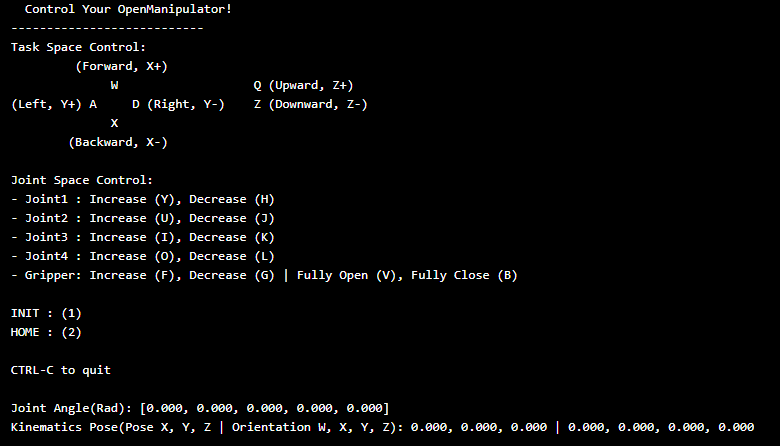
\includegraphics[width=\textwidth]{teleopkeyboard}
\caption{Fernsteuerung des OMX über die Tastatur}
\label{fig:teleopkeyboard}
\end{figure}
\begin{figure}[htb]
    \centering
    \begin{minipage}[t]{0.45\linewidth}
        \centering
        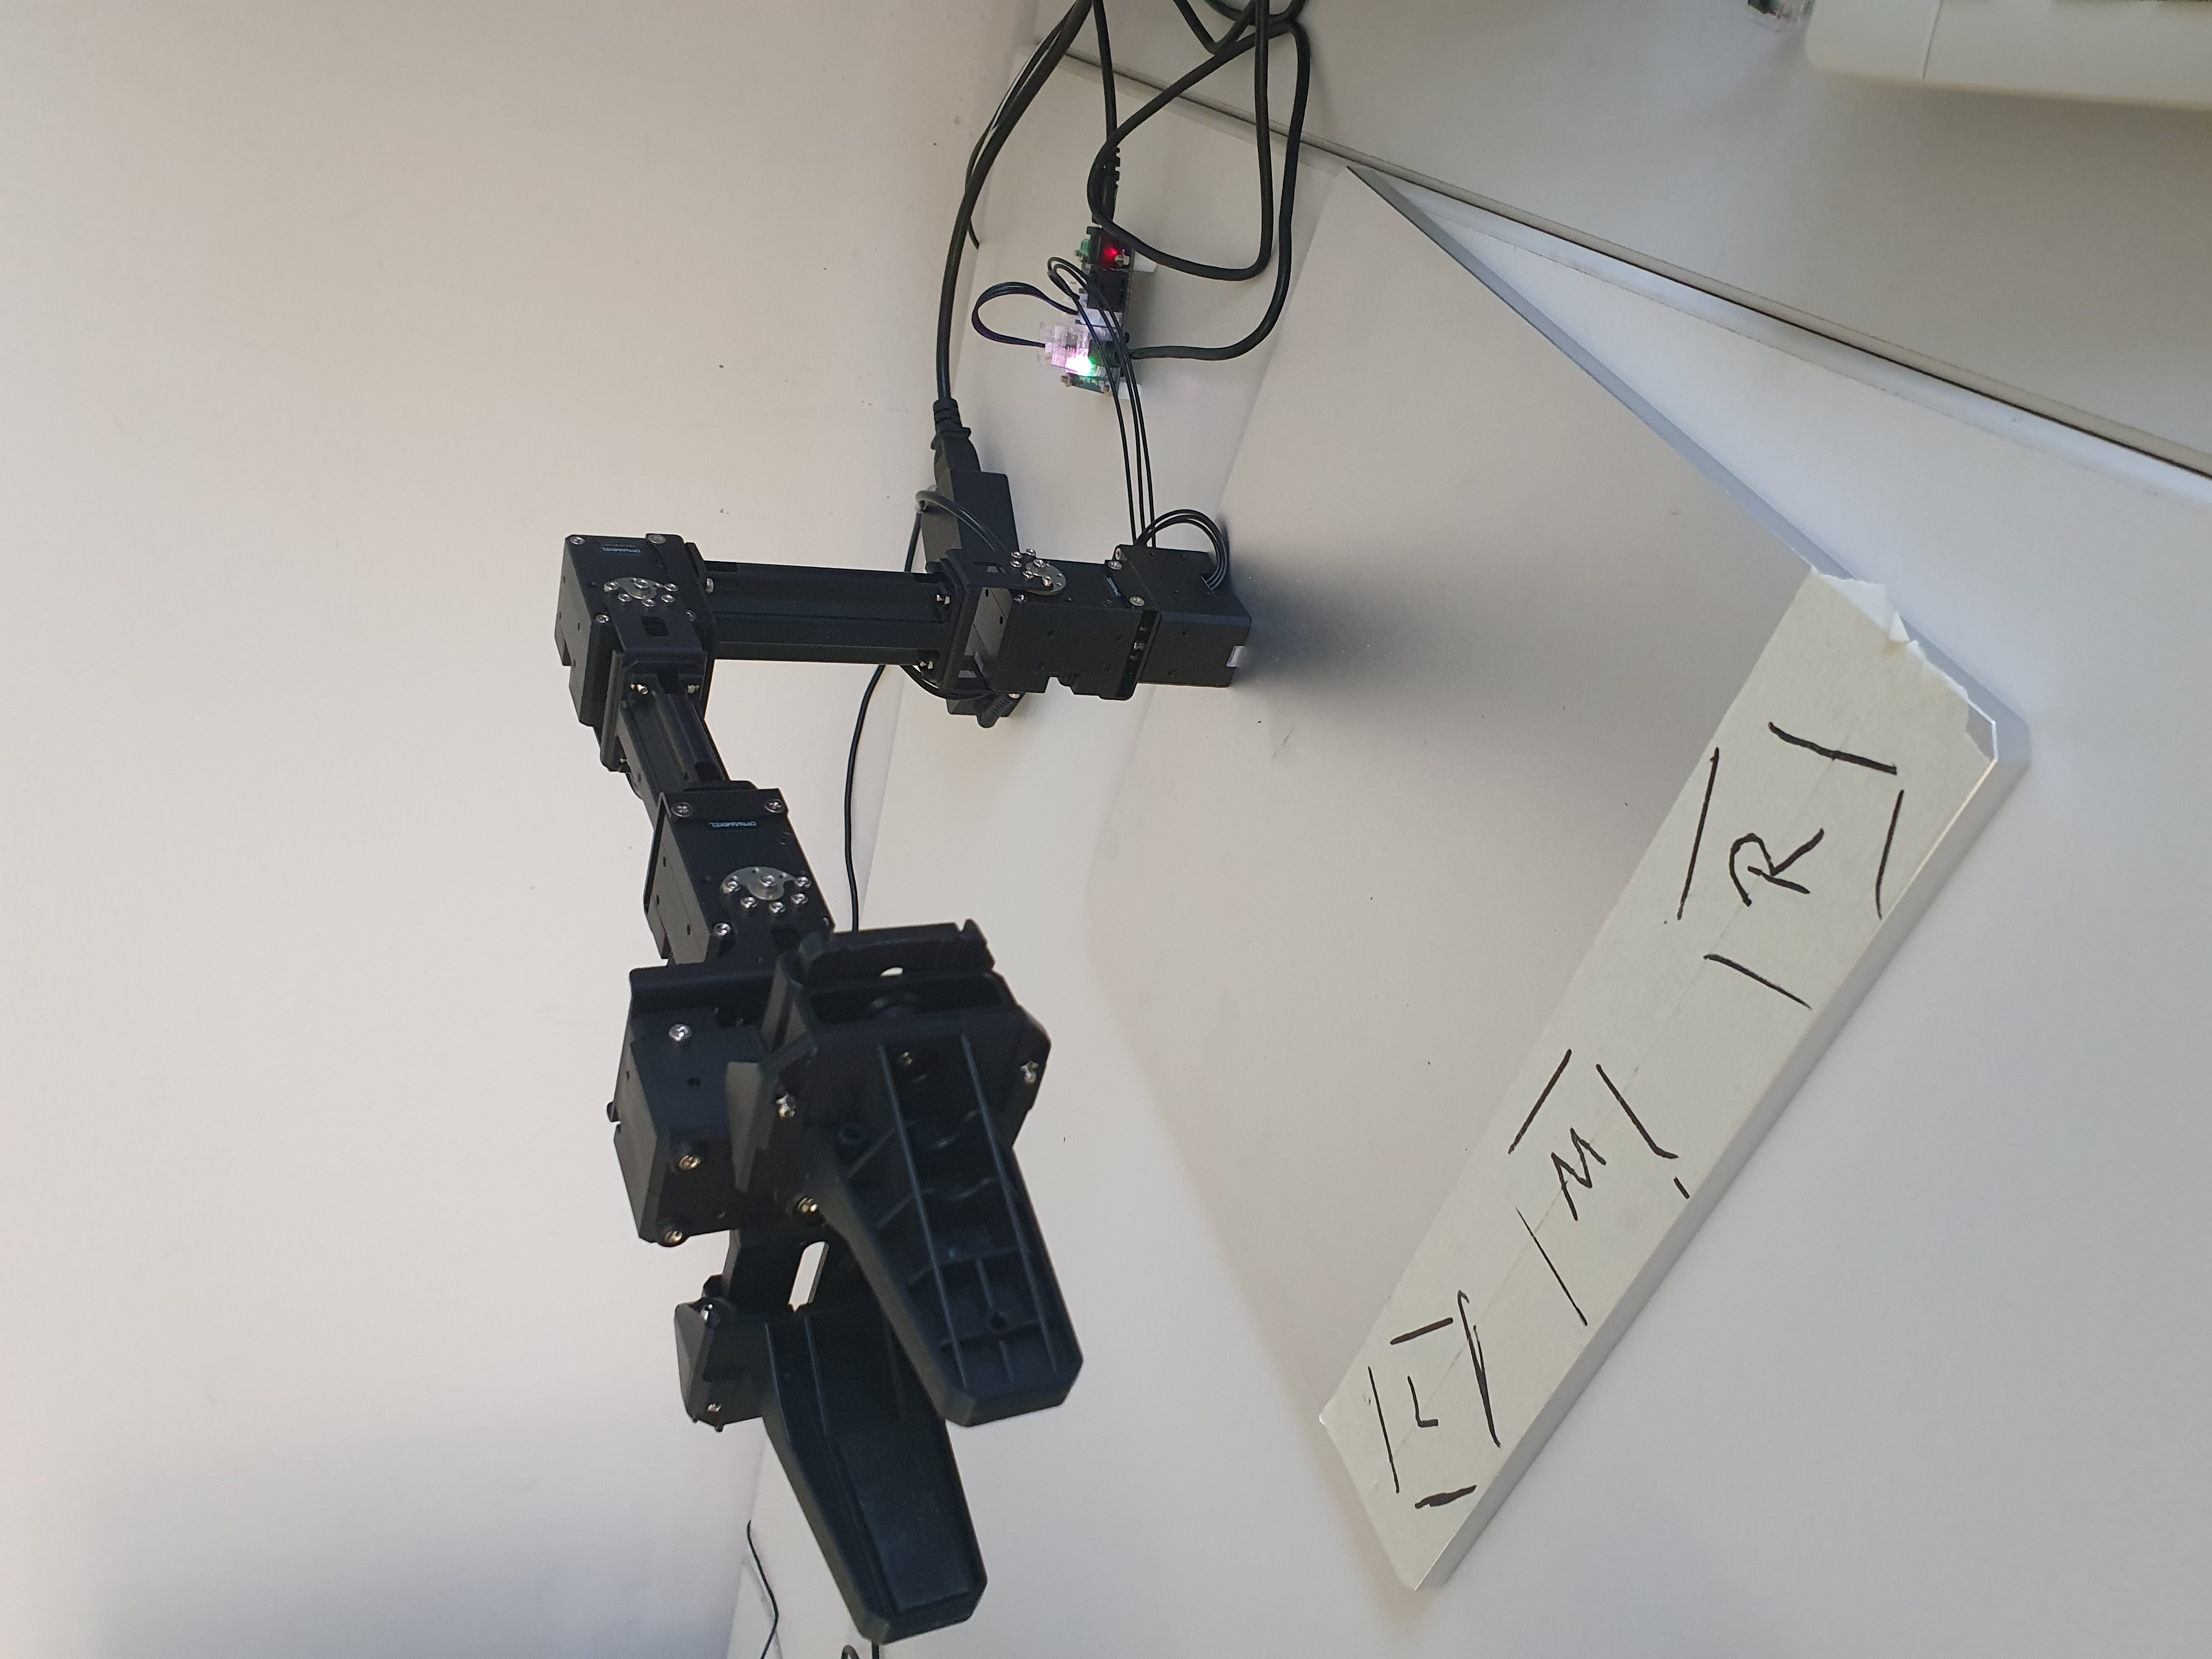
\includegraphics[width=\linewidth,keepaspectratio]{initpose}
    \end{minipage}% <- sonst wird hier ein Leerzeichen eingefügt
    \hfill
    \begin{minipage}[t]{0.45\linewidth}
        \centering
        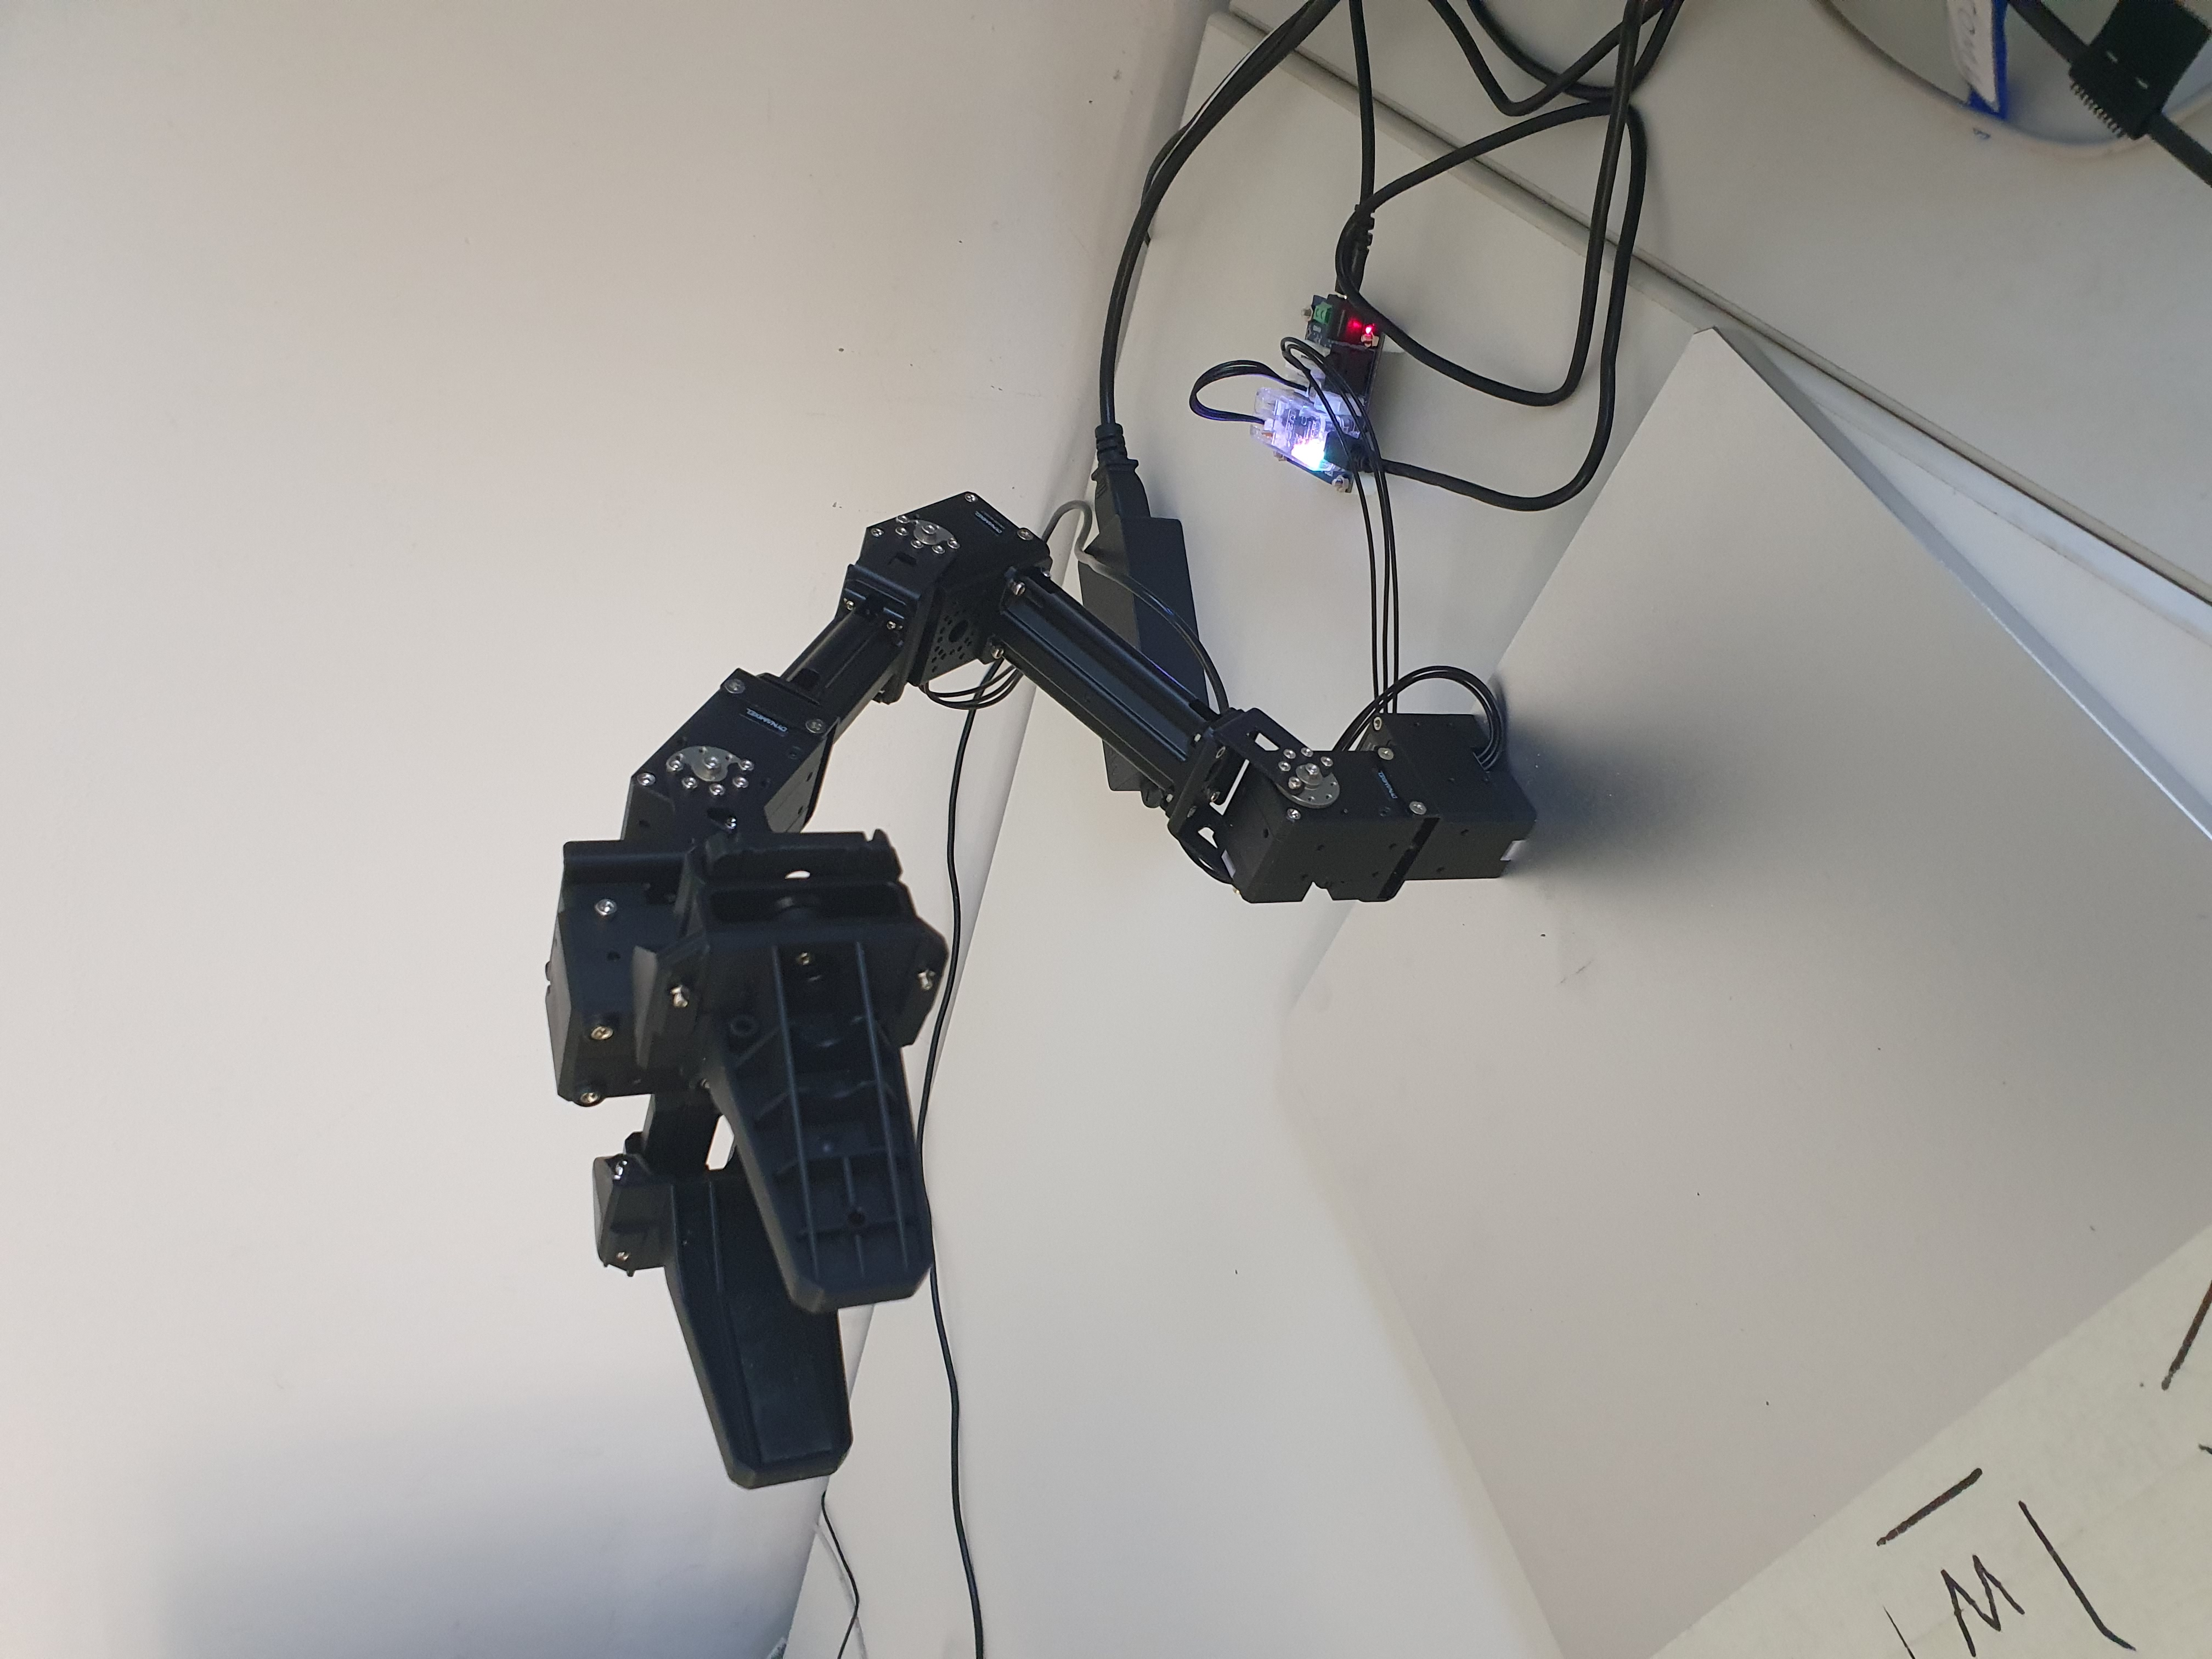
\includegraphics[width=\linewidth,keepaspectratio]{homepose}
    \end{minipage}
    \caption{Init (l.) und Home (r.) Pose der Tastatur Teleop}
    \label{fig:teleopposes}
\end{figure}



\subsection{PlanSys2}~\cite{plansys}\\
Für die Implementierung der in Abschnitt~\ref{konzept:nodes} genannten Funktionalitäten wird das Framework \ac{PlanSys2} genutzt.
Es übernimmt dabei alle Funktionalitäten: die Verwaltung der Daten zur Domäne und dem aktuellen Problem erfolgt über die domain-expert und problem-expert Nodes.
Die planer Node ist für die komplette Planung zuständig und die Executioner Node für die Ausführung des Plans.\\
Es müssen hier lediglich die Domäne erstellt sowie die tatsächliche Funktionalität der einzelnen Aktionen implementiert werden.
Das Wort Action im Namen der Nodes und den folgenden Kapiteln bezieht sich hier auf die Aktionen der Domäne, nicht auf \ac{ROS2} Actions.



\subsubsection{PDDL-Domain}
Beim erstellen der Domäne ist zu beachten, das \ac{POPF} nicht alle Funktionen unterstützt, die mit PDDL beschrieben werden können.
Dies beinhaltet unter anderem existentielle sowie negative Vorbedingungen.
Die vollständige Liste ist auf~\ref{popfpddlsupport} zu finden.\\
Für den Blockworld Teil der Domäne gibt es zunächst den Typ \verb|box| und Prädikate, die das Stapeln von Blöcken darstellen.
Dies umfasst das Verhältnis von Blöcken aufeinander (\verb|(box_on ?b_above ?b_below - box)|) sowie ob ein Block der oberste eines Stapels und damit frei zum bewegen ist (\verb|(clear ?b - box)|).
Als Aktionen werden das Nehmen sowie Ablegen eines Blocks benötigt.
Da in den Bedingungen und Effekten einer Aktion nur mit Parametern gearbeitet werden kann, welche auch Parameter der Aktion selbst sind, wird hier weiter aufgeteilt in Nehmen/Ablegen eines Blocks von/auf einen anderen Block sowie von/auf einen leeren Stapel.
Für das Bewegen von Blöcken ergeben sich die 4 Aktionen \verb|GRAB, PLACE, STACK, UNSTACK|.\\
Während für das reine Stapeln der Blöcke die exakte Position dieser nicht wichtig ist, wird diese jedoch für den Greifer benötigt, welcher vor diesen Aktionen an die richtige Stelle bewegt werden muss.
Hier werden die weiteren Typen \verb|location| und \verb|stack| sowie die Prädikate \verb|(box_at ?b - box ?l - location)|,\\ \verb|(gripper_at ?g - gripper ?l - location)|,\\ \verb|(location_above ?l_above ?l_below - location)| und\\ \verb|(is_base_loc ?l - location ?s - stack)| eingeführt.\\ \\
Das Prädikat \verb|clear| ist notwendig, da \ac{POPF} weder existentielle noch negative Vorbedingungen unterstützt.
Es wird genutzt um zu überprüfen, ob ein Block der oberste eines Stapels ist, was es ermöglicht diesen zu nehmen oder einen anderen auf diesem abzulegen.
Durch existentielle und negative Vorbedingungen könnte dies für die Aktion den Block B zu greifen, durch eine Bedingung der Form ''es existiert kein Block C für den gilt:( box\_on C B)'' ersetzt werden. \\ \\
Da alle Aktionen eine Dauer haben und \ac{PlanSys2} auch nur diese unterstützt, werden alle Aktionen als \verb|durative-action| modelliert.
Es wird jeder Aktion eine Dauer zugeordnet (\verb|:duration (= ?duration 0.25)|) welche auch für Metriken genutzt werden kann.
Zusätzlich bekommen Bedingungen und Effekte einen temporalen Zusatz: \verb|at start| und \verb|at end| können sowohl für Bedingungen als auch Effekte benutzt werden, um festzulegen zu welchem Zeitpunkt der Aktion diese Bedingung zutreffen oder der Effekt eintritt.
Für Bedingungen gibt es außerdem \verb|over all| damit eine Bedingung über die komplette Dauer der Aktion zutreffen muss damit sie gültig ist.\\
Da Bedingungen dadurch nicht mehr strikt vor Ausführung der Aktion gelten müssen, wird das Schlüsselwort \verb|:precondition| zu \verb|:condition| geändert.
Im aktuellen Szenario wird \verb|over all| dafür genutzt, allen Block-Aktionen die Bedingung zu geben, dass sich der Greifer über die komplette Zeit an der gleichen Stelle wie der entsprechende Block befinden muss.\\
Nur in der \verb|MOVE-GRIPPER| Aktion wird \verb|at start| für einen Effekt genutzt:\\
\verb|(at start(not (gripper_at ?g ?l_from)))|.\\
Sobald die Aktion beginnt befindet sich der Greifer nicht mehr an der Ausgangsposition und erst am Ende der Aktion wird die neue Position als Fakt gesetzt:\\
\verb| (at end(gripper_at ?g ?l_to))|.
Würden beide Effekte erst am Ende der Aktion eintreten, würde der Planer mehrere \verb|MOVE-GRIPPER| Aktionen parallel ausführen (s. Abbildung~\ref{fig:tempgrippereffect}).
Dies ist zum einen physisch nicht möglich, hinterlässt die Welt aber auch in einem ungültigen Zustand, da der Greifer sich dann an mehreren Positionen gleichzeitig befinden würde.

\subsubsection{Action Nodes}
Obwohl in der Domäne mehr als 2 Aktionen beschrieben sind, beschränken sich die ausgeführten Aktionen auf ein Bewegen des OMX sowie die Kontrolle des Greifers.
Für diese wird jeweils eine Node erstellt.
Damit diese Nodes von \ac{PlanSys2} genutzt werden können, müssen sie von der Basisklasse \verb|plansys2::ActionExecutorClient| erben.
Da diese von \ac{PlanSys2} nur in C++ zur Verfügung gestellt wird, müssen auch die Aktionen in C++ implementiert werden.\\
In jeder Aktion muss die Methode \verb|void do_work()| implementiert werden.
Diese wird mit einem bestimmten Zeitintervall aufgerufen während die Aktion aktiv ist.
Das Intervall wird im Konstruktor gesetzt (s. Zeile~\ref{code:line:nodeintervall} in~\ref{code:gripperactionnode}).
Das Mapping einer Node zu einer Aktion erfolgt durch das Setzen des Parameters \verb|action_name| nach dem Erstellen der Node (s. Zeile~\ref{code:line:actionname} in~\ref{code:gripperactionnode}).

\subsubsection{Control Gripper Aktion}
Die Logik Node zur Steuerung des Greifers wird in der Klasse \verb|ControlGripperAction| (s.~\ref{code:gripperactionnode}) implementiert.
Da es vom OMX kein Feedback gibt, ob oder wann etwas gegriffen wurde, wird die Aktion mit einer fixen Wartezeit implementiert: wenn die Aktion gestartet wird, wird ein Request zur Steuerung des Greifers erzeugt (s. Zeile~\ref{code:line:gripperrequest} in~\ref{code:gripperactionnode}) und gesendet und nach einer bestimmten Zeit die Aktion beendet.
Um unnötige Aufrufe der Methode während des Wartens zu verhindern wird die Wartezeit über das Zeitintervall zur Ausführung der Node gesetzt.
Die Aktion wird hierdurch immer beim 2.\ Aufruf der Methode \verb|do_work| beendet.\\
Zum Senden des Requests wird ein \ac{ROS2} Client für den Service \verb|goal_tool_control| mit dem Typ \verb|open_manipulator_msgs::srv::SetJointPosition| erstellt. 
Um sowohl die Aktionen zum Öffnen sowie Schließen des Greifers mit einer Node implementieren zu können wird ein Parameter eingeführt, welcher über den Konstruktor gesetzt wird und die Bewegung des Greifers bestimmt.
Für jede Aktion wird eine Node mit entsprechenden Parametern erzeugt.
Diese Nodes werden alle einem \verb|MultiThreadedExecutor| hinzugefügt. Dadurch können alle Nodes gemeinsam gestartet werden und laufen in einem Prozess, sind durch mehrere Threads aber unabhängig voneinander.

\subsubsection{Move Gripper Aktion}
Die Logik Node zur Bewegung des OMX wird in der Klasse \verb|MoveGripperAction| (s.~\ref{code:moveactionnode}) implementiert.
Insgesamt umfasst dies das Senden des Bewegungsrequests an den vom OMX-Controller erstellten Service \verb|goal_task_space_path_position_only| mit dem Typ \verb|open_manipulator_msgs::srv::SetKinematicsPose| (s. Zeile~\ref{code:line:poseclient} in\ref{code:moveactionnode}) sowie das Beenden der Aktion wenn der OMX an der Zielposition angekommen ist.
Ob die Bewegung beendet ist wird über den im Topic \verb|states| gesendeten Bewegungsstatus geprüft.
Dieser kann die beiden Werte \verb|IS_MOVING| und \verb|STOPPED| annehmen.
Der aktuelle Status wird mit dem letzten empfangenen verglichen: war der letze Status \verb|IS_MOVING| und der aktuelle \verb|STOPPED|, waren wir in einer Bewegung, die jetzt beendet ist.\\
Um die Zielkoordinaten der Bewegung zu erhalten, muss der String Parameter der Aktion in Zahlenwerte konvertiert werden.
Zunächst werden aus dem String, welcher im Format \verb|s<Nummer des Stapels>l<Höhe innerhalb eines Stapels>| vorliegt, die 2 Integerwerten mit Hilfe einer regular Expression extrahiert.
Diese werden im 2.\ Schritt über Maps zu Y und Z Koordinaten konvertiert.
Die X Koordinate ist im Rahmen dieser Arbeit fest auf den Wert 0,25 gesetzt.\\
Um eine kollisionsfreie Bewegung sicherzustellen findet diese nicht direkt von der aktuellen zur Zielposition statt.
Stattdessen werden mehrere Zwischenpositionen errechnet und entsprechende Bewegungen zuerst ausgeführt.
Zunächst wird der OMX bei gleichbleibenden X und Y Koordinaten auf eine Z Koordinate von 0,25 bewegt.
Dies entspricht eine Höhe in der keine Blöcke liegen können.
Die zweite Zwischenposition bleibt auf der gleichen Höhe (Z Koordinate 0,25) und bewegt sich zur X und Y Koordinate der Zielposition.
Diese Zwischenposition befindet sich exakt oberhalb der Zielposition, sodass eine vertikale Bewegung zur Zielposition ohne Kollision möglich ist.\\
Diese Zwischenpositionen werden übersprungen, wenn die aktuelle Position des OMX bereits dem korrekten Stapel der Zielposition entspricht.
Hierbei werden die aktuellen Koordinaten auf 2 Dezimalstellen gerundet.\\
Für alle benötigten Positionen wird ein Request erzeugt und einer Queue hinzugefügt.
Der Auslöser, den nächsten Request zu senden ist jeweils das Ende der vorherigen Bewegung.\\
Um Zugriff auf die aktuelle Position des OMX zu erhalten wird ein weiterer Subscriber für das Topic \verb|kinematics_pose| benötigt, welches eine Message vom Typ\\
\verb|open_manipulator_msgs::msg::KinematicsPose| veröffentlicht.\\
Um eine Beschädigung der Motoren zu vermeiden, soll die Bewegung bei einer Kollision abgebrochen werden.
Hierfür sind zwei Teile nötig: die Kollisionserkennung sowie das Abbrechen der Bewegung.
Für die Kollisionserkennung wird der Stromverbrauch der einzelnen Motoren genutzt.
Dieser steigt, wenn der Motor mehr Leistung bringen muss, wenn versucht wird sich gegen ein Hindernis zu bewegen.\\
Dieser ist in der Message des Topics \emph{joint\_states} als \emph{effort} enthalten.
Die letzten $x$ Werte (konfigurierbar über die Variable \emph{EFFORT\_COUNT}, standardmäßig 10) werden für jeden Motor gespeichert (s. Zeile~\ref{code:line:effortsaving} in \ref{code:moveaction}) und ausgewertet (s. Zeile~\ref{code:line:efforteval} in \ref{code:moveaction}).
Die Werte jedes Motors werden einzeln ausgewertet.
Es wird das Maximum und das Minimum der Werte genommen und geprüft ob die absolute Differenz größer als der festgelegte Grenzwert (konfigurierbar über die Variable \emph{EFFORT\_THRESHOLD}, standardmäßig 500) ist.
Ist dies für mindestens einen Motor der Fall gilt die Aktion als fehlgeschlagen und der entsprechende Status wird zurückgegeben (s. Zeile~\ref{code:line:effortfail} in \ref{code:moveaction}).
Eine fehlgeschlagene Aktion resultiert gleichzeitig in einem fehlgeschlagenen Plan.
Ein Abbrechen der Aktion verhindert jedoch nicht, dass der OMX versucht das aktuelle Bewegungsziel zu erreichen.
Es wird ein neues Bewegungsziel erstellt, das sich an der aktuellen Position befindet.


\subsubsection{Package}
- pkg build config\\
Alle erstellten Komponenten werden in einem eigenen \ac{ROS2} Package gebündelt.
Dies umfasst die C++ Dateien für die Aktionen sowie die Domänendatei.
Es wurde eine Launch Datei erstellt um das komplette System über einen Befehl starten zu können.
In der Launch Datei wird zum einen \ac{PlanSys2} und zum anderen die Nodes für alle Aktionen gestartet.
Weiterhin wird hier festgelegt, welche Domäne genutzt wird.\\
Das Package enthält außerdem eine Readme Datei in der die nötigen Schritte beschrieben sind um das gesamte System, einschließlich OMX, zu starten.
Weiterhin wurden mehrere Problemszenarien erstellt, die sowohl als \ac{PDDL} Datei als auch als Befehle für das \ac{PlanSys2} Terminal zur Verfügung stehen.

\subsection{Praktische Anwendung}
Um das System praktisch anwenden zu können wurden mehrere farbige Würfel aus LEGO gebaut (s. Abbildung~\ref{fig:legocubes}).
Auf der Basisplatte des OMX wurden die Positionen der 3 Stapel markiert.
\subsubsection{PlanSys2 Terminal}
Das \ac{PlanSys2} Terminal ist eine separate Node, welche es ermöglicht, das System durch Eingabe über die Konsole zu steuern.
Die wichtigsten Befehle sind hierbei \verb|get|, \verb|set| und \verb|run|.
Mit \verb|get| können die Typen, Prädikate und Aktionen der geladenen Domäne sowie des aktuellen Problems angezeigt werden (s. Abbildung~\ref{fig:plansysterminal}).
Der \verb|set| Befehl wird genutzt, um das aktuelle Problem zu verändern.
Es können Instanzen, Prädikate sowie das Ziel erstellt und geändert werden.
Über den Befehl \verb|run| lässt sich der Plan für das aktuelle Ziel ausführen.
Es ist auch möglich nur einen Plan zu suchen, ohne ihn direkt auszuführen.
Dies ist mit \verb|get plan| möglich (s. Abbildung~\ref{fig:terminalplan}).\\
Während der Ausführung eines Plans wird im Terminal die aktuelle Aktion sowie dessen Fortschritt (gesteuert über den Feedback Kanal innerhalb der Aktion) angezeigt.
\subsubsection{Abstürze und Fehlersuche}
Während der Ausführung eines Plans kam es wiederholt zu Abstürzen der \ac{PlanSys2} Node.
Diese Abstürze verhinderten eine vollständige Ausführung des Plans und erforderten einen Neustart des \ac{PlanSys2}-Systems.
Der Absturz erfolgte immer mit einem Exit Code 11, der auf ein SEGMENTATION FAULT hinweist.
Um die Stelle des Absturzes zu finden wurde \ac{PlanSys2} zunächst in der distributed anstelle der Monolithic Version gestartet.
Hierdurch werden alle Nodes in eigenen Prozessen gestartet.
Dies ermöglichte ein Eingrenzen auf die Executor Node.\\
Für das weitere Debugging wurde der GNU Project Debugger (GDB) sowie xterm (musste separat installiert werden) genutzt.
In der Launch-Datei für den Executor wurde der Node \verb|prefix=['xterm -e gdb -ex run --args'],| hinzugefügt, um beim Start der Node auch eine Debugging-Session zu starten.\\
Über den backtrace nach einem Absturz wurde die Methode\\\verb|ActionExecutor::request_for_performers()| als Ursache für den Absturz identifiziert.
Innerhalb dieser Methode wurde das Problem in der Zeile\\\verb|action_hub_pub_->publish(msg);| gefunden.
Zum Zeitpunkt eines Absturzes hatte die Variable \verb|action_hub_pub_| den Wert \verb|null|.
Um den Absturz zu verhindern wurde ein \verb|null|-Check implementiert.
Obwohl dieser dafür sorgt, dass einige Messages nicht gesendet werden, führte diese Änderung zu keinen offensichtlichen Nebenwirkung und Pläne werden normal ausgeführt.

\begin{figure}[ht!]
    \centering
    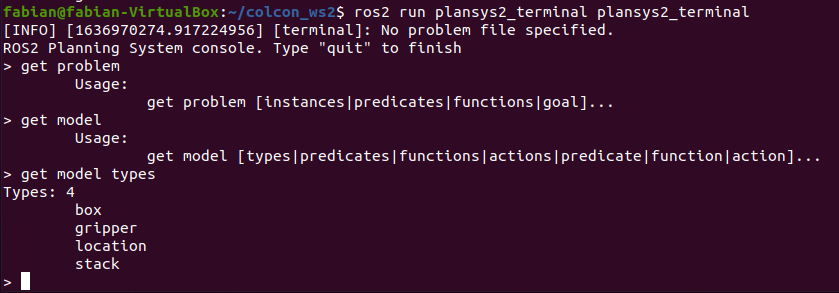
\includegraphics[width=\textwidth]{plansys2terminal}
    \caption{\ac{PlanSys2} Terminal mit Abfrage der Typen des geladenen Models}
    \label{fig:plansysterminal}
\end{figure}

\begin{figure}[ht!]
    \centering
    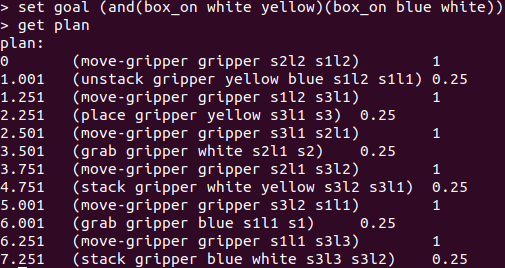
\includegraphics[width=\textwidth]{simple_plan}
    \caption{Ausgabe eines Plans in \ac{PlanSys2} Terminal}
    \label{fig:terminalplan}
\end{figure}
\section{Ergebnis}
\subsection{Zusammenfassung}
Der Zusammenbau erfolgte ohne größere Probleme.
Die beschriebenen Details, die leicht zu übersehen sind, lassen sich auch im Nachhinein ohne großen Aufwand beheben oder korrigieren.
Durch die verfügbaren Installations-Skripte gab es auch softwareseitig keine Hindernisse für einen schnellen Einstieg.
Auch wenn zu Beginn dieser Arbeit noch keine offizielle Unterstützung von \ac{ROS2} Foxy vorhanden war, konnte anhand der Anleitung für ältere \ac{ROS2} Distributionen alles zum laufen gebracht werden.
Durch die Kombination der \ac{ROS2} Foxy Tutorials sowie der OpenMANIPULATOR-X API Dokumentation ließen sich auch ohne Vorkenntnisse gute Fortschritte machen.
\subsection{Ausblick}
\subsubsection{MoveIt}
Um den in der dieser Arbeit verwendeten Ansatz der Bewegungsplanung robuster und dynamischer zu machen, empfiehlt sich die Implementierung der Bibliothek MoveIt\footnote{MOVEIT URL}.
Zum Zeitpunkt der Bearbeitung wird diese vom OpenMANIPULATOR-X beim Betrieb mit \ac{ROS2} Foxy allerdings noch nicht offiziell unterstützt.\\
MoveIt bietet mittels virtueller Szenen die Möglichkeit, effiziente und kollisionsfreie Wege für die Bewegung des OpenMANIPULATOR-X zu planen und auszuführen.
In der virtuellen Szene befindet sich sowohl ein Modell des Roboters als auch aller relevanten Hindernisse.
Wird eine Bewegung zu einer Position angefordert, kann der generierte Pfad auf potenzielle Kollisionen mit Objekten der Szene überprüft werden.
\subsubsection{Vorschläge für Übungen in der Lehre}
Um die Verwendung des OpenMANIPULATOR-X in der Lehre näher zu bringen, gibt es in dem für diese Arbeit entstandenen Package mehrere Stellen, an denen angesetzt werden kann.\\
Grundsätzlich lassen sich diese in folgende Bereiche aufteilen:
\begin{itemize}
\item \ac{ROS2}
\item Domäne und Problem in PDDL
\item ...
\end{itemize}
Für jeden dieser Bereiche besteht die Möglichkeit die Aufgaben in die folgenden Richtungen zu führen:
\begin{itemize}
\item Fehlersuche mit sinnvoll platzierten Fehlern
\item Erkennen und Korrigieren weggelassener Abschnitte, welche durch das Verstehen des Codes erkannt werden können
\item die Anpassung des Codes an ein ähnliches Szenario
\end{itemize}
Ein Beispiel für die Domäne ist, den Effekt der \verb|MOVE-GRIPPER| Aktion, der die Startposition löscht, erst am Ende der Aktion auszuführen, was dazu führt, dass zum Start des Plans alle nötigen Bewegungen gleichzeitig ausgeführt werden.\\
Eine Aufgabe für das Schreiben/Anpassen eines Problems in PDDL, welche sich anbietet, ist eine vorgegeben Problemdatei, welche nur die grundlegende Struktur über Stapel und Positionen enthält, so zu erweitern, dass eine von mehreren möglichen, vorgegebenen Varianten von gestapelten Blöcken beschreibt.
Die Aufgabe kann dadurch erleichtert werden, dass das gegebene Problem bereits eine bestimmte Stapelung von Blöcken darstellt und nur angepasst werden muss.\\
Für alle Aufgaben, die PDDL betreffen, bietet es sich an, VS-Code mit dem PDDL-Plugin zu nutzen, um schnelle Iterationen und eine Visualisierung der Pläne zu ermöglichen.
%
\section{Abschnitt} 
Hier soll eine kurze Einführung erfolgen, die den Zusammenhang des Kapitels zur Arbeit herstellt.

Generelle Hinweise:

\begin{itemize}
\item eindeutige Begrifflichkeit verwenden
\item auf logische Herleitung der Argumentation achten
\end{itemize}

Ein Hauptabschnitt - idealerweise sollten keine Abschnitte leer sein.

\subsection{Unterabschnitt}
Ein Unterabschnitt - idealerweise sollten keine Abschnitte leer sein.

\subsubsection{Unterunterabschnitt}
Ein Unterunterabschnitt - idealerweise sollten keine Abschnitte leer sein.

\section{Einfache Formatvorlagen}

\textbf{Das ist fett gedruckter Text}.

\textit{Das ist kursiver Text}.


Auflistungen sind oft hilfreich für die Strukturierung:
\begin{itemize}
    \item Erster Eintrag
    \item Zweiter Eintrag
\end{itemize}

Nummerierte Aufzählungen sind oft hilfreich für Reihenfolgen:
\begin{enumerate}
    \item Erster Eintrag
    \item Zweiter Eintrag
\end{enumerate}


\section{Zitieren und Referenzieren}

Beiträge in Fachzeitschriften wie \citet[12]{clemen1989combining} oder Konferenzartikel wie \citet[6]{he2017mask} werden auf diese Weise im Text zitiert. In anderen Fällen möchte man aber in Klammern zitieren \citep[10]{clemen1989combining}, auch mit mehreren Autoren (\citealp[3]{baumol1958warehouse}; \citealp[15]{clemen1989combining}; \citealp[12]{he2017mask}).

Die Seitenzahlen müssen angegeben werden \citep[28]{chollet2018deep}. Bezieht sich das Zitat auf eine Textstelle, die sich über mehrere Seiten streckt, so sind diese entsprechend anzugeben: \citet[28-29]{chollet2018deep} bzw. \citet[28-35]{chollet2018deep}

So wird eine Webquelle zitiert: \citet{shiny1}. Es kann bei kurzen Informationen im Internet aber auch reichen die Adresse\footnote{\url{https://shiny.rstudio.com/tutorial/written-tutorial/lesson1/}} als Fußnote einzubetten.

Bei einem direkten Zitat muss der zitierte Text originalgetreu wiedergegeben werden. Rechtschreibfehler oder eine veraltete Orthographie werden unverändert wiedergegeben. „Der zitierte Text steht immer in Anführungszeichen"\ \citep[28]{chollet2018deep}. 

So werden andere Teile der Arbeit referenziert: Kapitel \ref{einleitung}, Gleichung \ref{eq:1} zeigt...

So verweisen wir auf eine Fußnote \footnote{dies ist eine Fußnote}.

\section{Abbildungen}

Abbildungen erfordern das package \textit{graphicx}. 
Idealerweise verwendet man Vektorgrafiken oder hochaufgelöste Bitmaps. 
Eine gute Variante ist das Verwenden von PDFs.

\begin{figure}[h]
    \centering
    
\includegraphics[width=0.3\textwidth]{figs/2015_10_05_THB_FB-IM_Logo_RGB.pdf}
    \caption{Siegel der Universität}
    \label{fig:my_label}
\end{figure}


\section{Tabellen}

Die Tabular-Umgebung gibt die Anzahl Spalten an, deren Orientierung, Breite und evtl. Zwischenlinien. 


\begin{table}[ht]
    \centering
    \caption{Meine Tabelle}
        \begin{tabular}{ cccc } 
        \toprule
        col1 & col2 & col3 \\
        \midrule
        \multirow{3}{4em}{Multiple row} & cell2 & cell3 \\ 
        & cell5 & cell6 \\ 
        & cell8 & cell9 \\ 
        \bottomrule
    \end{tabular}
    \label{tab:countries}
\end{table}

\section{Formeln}

\begin{equation}
    \sum_{i=1}^N x_i
    \label{eq:1}
\end{equation}

\section{Abkürzungen}
Bei der ersten Verwendung wird die Abkürzung eines Fachbegriffs wie zum Beispiel \ac{ML} eingeführt und daher ausgeschrieben. Bei der zweiten Verwendung der Abkürzung \ac{ML} ist dies nicht mehr nötig. Die Abkürzungen sind in dem Abschnitt \textit{Definition der Abkürzungen} einzupflegen. Das Abkürzungsverzeichnis ist alphabetisch anzuordnen. Bleibt das Abkürzungsverzeichnis leer, so kann dieser Abschnitt (Zeilen 164-173 im main.tex) gelöscht werden.


\section{Fazit}
In der Schlussfolgerung sollen

\begin{itemize}
\item die Themenstellung
\item der gewählte Ansatz
\item die Ergebnisse der Arbeit
\item eine kritische Stellungnahme/Einschätzung
\item nächste Schritte
\end{itemize}
deutlich werden.

Hinweis:
Die Schlussfolgerung sollte mit der Zusammenfassung bzw. dem Abstract und der Einleitung abgeglichen werden. Es sollte immer eine Zusammenfassung der wesentlichen Er-kenntnisse der eigenen Arbeit sein, die den Forschungsbeitrag darstellt. Der Umfang der Schlussfolgerung sollte ähnlich wie die Einleitung ca. 5 \% der gesamten Arbeit betragen.


%%%%%%%%%%%%%%%%%%%%%%%%%%%%
%% Literaturverzeichnis wird 
%% automatisch eingefügt
%%%%%%%%%%%%%%%%%%%%%%%%%%%%
\clearpage
\lhead{}
\printbibliography
\addcontentsline{toc}{section}{\bibname}


%%%%%%%%%%%%%%%%%%%%%%%%%%%%
%% Anhang (optional) 
%%%%%%%%%%%%%%%%%%%%%%%%%%%%
\clearpage
\appendix
\section{Quellcode} % Bei englischsprachiger Arbeit anzupassen auf: Appendix A
\subsection{Planungsdomäne}
\lstinputlisting[language=pddl,label=lst:domain]{apdx/domain.pddl}
%\subsection{Gripper Package Launch Datei}
%\lstinputlisting[language=Python]{apdx/blockworld_gripper_launch.py}
\subsection{Move Gripper Action Node}
\lstinputlisting[language=C++,label=lst:move_action]{apdx/move_gripper_action_node.cpp}
\subsection{Control Gripper Action Node}
\lstinputlisting[language=C++,label=lst:gripper_action]{apdx/control_gripper_action_node.cpp}
%%%%%%%%%%%%%%%%%%%%%%%%%%%%
%% Versicherung zur Leistungserbringung 
%% ist auf der Webseite des 
%% Lehrstuhls zu finden.
%%%%%%%%%%%%%%%%%%%%%%%%%%%%

\end{document}